%%%%%%%%%%%%%%%%%%%%%%%%%%%%%%%%%%%%%%%%%%%%%%%%%%%%%%%%%%%%%%%%%%%%%%
% James Bueghly's Northwestern Ph.D. Thesis
% Department of Physics and Astronomy
% CMS Run II Higgs to Z+gamma Analysis
%%%%%%%%%%%%%%%%%%%%%%%%%%%%%%%%%%%%%%%%%%%%%%%%%%%%%%%%%%%%%%%%%%%%%%

%%%%%%%%%%%%%%%%%%%%%%%%%%%%%%%%%%%%%%%%%%%%%%%%%%%%%%%%%%%%%%%%%%%%%%
% template from Northwestern Department of Mathematics
% nuthesis-template.tex - Miguel A, Lerma - 4/23/2018
%                         mlerma@math.northwestern.edu
%%%%%%%%%%%%%%%%%%%%%%%%%%%%%%%%%%%%%%%%%%%%%%%%%%%%%%%%%%%%%%%%%%%%%%

% The nuthesis class is based on % amsbook.cls.
\documentclass[12pt]{template/nuthesis}	
\usepackage{xcolor}

\author{James Bueghly}

\title{The Search for the Higgs Boson Decaying into a Z Boson and a Photon}

%\degree{DOCTOR OF PHILOSOPHY}  % Default: DOCTOR OF PHILOSOPHY

\field{Physics and Astronomy}            % Default: Mathematics

%\graduationmonth{June}         % The default is June or December
                                % depending on current date.

%\graduationyear{2003}          % Default: current year.


				% Use \includeonly to select the 
%\includeonly{chap1,chap2,...}	% chapters to include if you are 
				% using the \include command below.
				% This way you can latex only a the 
				% part you are working on, which 
				% is faster than latexing the entire 
				% thesis. 


\begin{document}
%	
%	THE BODY OF YOUR THESIS STARTS HERE
%

%%%%%%%%%%%%%%%%%%%%%%
% Some initial stuff %
%%%%%%%%%%%%%%%%%%%%%%

\frontmatter		% Preliminary pages start here.

\maketitle		% Produces the title page.

\copyrightpage		% Creates the copyright page.


% Abstract.
\abstract

Since its discovery in 2012 at the Large Hadron Collider (LHC), efforts have been made to measure and characterize the properties of the Higgs boson. 
Among these efforts have been searches for rare decays of the Higgs predicted by the standard model (SM) of particle physics. 
One such decay is the process \hzg, which has an expected branching fraction of $\mathcal{B}(\PH\to\PZ\gamma) = (1.57 \pm 0.09) \times 10^{-3}$ in the SM, 
assuming a Higgs boson mass of $m_\PH = \mH\GeV$.
This decay mode has not yet been experimentally observed, and its observation and measurement remains an important goal of Higgs physics research at the LHC.
In addition, a measurement of this decay mode at a rate deviating from the SM prediction would provide indirect evidence of new physics beyond the SM (BSM). 

This thesis presents a search for \hzg, where $\mathrm{Z}\to\ell^+\ell^-$ with $\ell=\mathrm{e}$ or $\mu$. The search is performed using a sample of proton-proton ($\mathrm{pp}$) collision data at a center-of-mass energy of $13~\mathrm{TeV}$, recorded by the Compact Muon Solenoid (CMS) experiment at the LHC, corresponding to an integrated luminosity of $138~\mathrm{fb}^{-1}$. 
Events are assigned to mutually exclusive categories, which exploit differences in both event topology and kinematics of distinct Higgs production mechanisms to enhance signal sensitivity. 
To detect a potential signal, fits are performed to the distributions of ${\ell^+\ell^-\gamma}$ invariant mass in each of these categories simultaneously.
The signal strength $\mu$, defined as the product of the cross section and the branching fraction [$\sigma(\mathrm{pp}\to\mathrm{H})\mathcal{B}(\mathrm{H}\to\mathrm{Z}\gamma)$] relative to the SM expectation, is found to be $\mu= 2.4\,\pm0.9$ for $m_\PH = \mH\GeV$. This measurement corresponds to $\sigma(\mathrm{pp}\to\mathrm{H})\mathcal{B}(\mathrm{H}\to\mathrm{Z}\gamma)=0.21\pm0.08~\mathrm{pb}$. The statistical significance of the observed excess of events is $2.7$ standard deviations. The observed (expected) upper limit at $95$\% confidence level (CL) on $\mu$ is $4.1$\,($1.8$). 
The ratio of branching fractions $\mathcal{B}(\mathrm{H}\to\mathrm{Z}\gamma)/\mathcal{B}(\mathrm{H}\to\gamma\gamma)$ is measured to be $1.5^{+0.7}_{-0.6}$, which agrees with the SM prediction at the 
$1.5$ standard deviation level. 


\acknowledgements	% Acknowledgements (optional).

Text for acknowledgments.

%\preface		% Preface (optional).
%
%This is the preface.


%% A few more optional pages (uncomment if needed)
%
%\listofabbreviations 
%
%This is the list of abbreviations (optional).
%
%\glossary
%
%This is the glossary (optional).
%
%\nomenclature
%
%This is the nomenclature (optional).
%
%% Note that the dedication text must be passed as an argument
%% of the \dedication command
%\dedication{This is the dedication (optional).}
%

\clearpage\phantomsection % needed for the hyperlinks to work correctly
\tableofcontents	% Table of Contents will be automatically
			% generated and placed here.

\clearpage\phantomsection % needed for the hyperlinks to work correctly
\listoftables		% List of Tables and List of Figures will be placed

\clearpage\phantomsection % needed for the hyperlinks to work correctly
\listoffigures		% here, if applicable (optional).



\mainmatter             % Actual text starts here.

%%%%%%%%%%%%%%%%%%%%%%%%%%%
% Actual text starts here %
%%%%%%%%%%%%%%%%%%%%%%%%%%%

% If there is an introduction it must be the first chapter

%\chapter{Introduction or Title of First Chapter}	% The first chapter.
%				% \chapter command is of the form
%				% \chapter[..]{..} or \chapter{..} where
%	... text ...		% {chapter heading} and [entry in table of
%				% contents].
%\section{First section of chapter 1}
%				% IMPORTANT: If your chapter heading consists
%				% of more than one lines, it will be auto-
%	... text ...		% matically broken into separate lines.
%				% However, if you don't like the way LaTeX
%				% breaks the chapter heading into lines, use
%\section{Another section}	% `\newheadline' command to break lines.
%				% Never use \\ in sectional (e.g., chapter,
%	... text ...		% section, subsection) headings.
%
%\chapter{Title of Second Chapter}	% Chapter 2.
%
%	... text ...
%
%\section{First section of chapter 2}
%
%	... text...
%
%\subsection{A subsection}
%
%	... more text ...
%
%\subsubsection{A subsubsection}
%
%	... more text ...


% Alternatively, you may write the chapters in separate
% files, say chap1.tex, chap2.tex, etc., and include them 
% with commands:

%\include{chap1}

%\include{chap2}

% The command \includeonly above allows to include a selected 
% set of chapters only.


\chapter{Introduction}

The standard model (SM) of particle physics is one of the most successful physics theories in history. It describes all of the fundamental particles we currently know in our universe, including the ways in which those particles interact with one another. Since its development in the second half of the twentieth century, the SM has been extensively tested through many measurements by numerous experiments. The Large Hadron Collider (LHC) was built with the goal of further testing the SM, while also searching for possible beyond the SM (BSM) physics at groundbreaking energy scales. One of the main goals of the LHC was to search for and observe the Higgs boson, a critical piece of the SM associated with the origin of particle mass.

Since the discovery of the Higgs boson~\cite{Aad_2012,Chatrchyan_2012,CMS:2013btf} at the LHC, an extensive program of measurements~\cite{PhysRevD.98.030001} has been undertaken to determine its properties and couplings to different types of particles and to assess whether these properties are consistent with those predicted by the SM. With the successful running of the LHC, large data samples of proton-proton ($\Pp\Pp$) collisions at $\sqrt s = 13\TeV$ have been accumulated, increasing the sensitivity to rare decays of the Higgs boson. 
Such decays also provide probes for possible contributions arising from BSM physics and include the process 
\hzg~\cite{Abba96, Chen12, Htollg-FB-Sun, Passarino, Campbell_2013hz, Degrassi:2019yix, Low:2011gn}.

Figure \ref{fig:fey} shows Feynman diagrams for the key SM contributions to the \hzg{} decay process. 
Experimentally, the final state resulting from $\PZ \to \ell^+ \ell^-$ ($\ell = \Pe$ or $\mu$) is the most accessible, since the leptons are highly distinctive, well-measured, and provide a means to trigger the recording of the events. 
\begin{figure*}[!b]
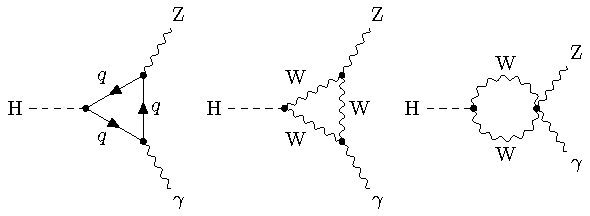
\includegraphics[width=0.9\textwidth]{fig/intro/Figure_001.pdf}
	\caption{Feynman diagrams for \hzg{} decay.} \label{fig:fey}
\end{figure*}
In the SM, the expected branching fraction for \hzg{} is $\mathcal{B}(\PH\to\PZ\gamma) = (1.57 \pm 0.09) \times 10^{-3}$, assuming a Higgs boson mass of $m_\PH = \mH\GeV$. This branching fraction is comparable to $\mathcal{B}(\PH\to\gamma\gamma)  = (2.27 \pm 0.04) \times 10^{-3}$~\cite{LHC-YR4,CMS:2021kom}. The value $m_\PH=\mH \pm 0.14\GeV$ is taken from the most recent Compact Muon Solenoid (CMS) Higgs boson mass measurement~\cite{CMS:2020xrn}, which uses the combination of $\PH\to\gamma\gamma$ and $\PH\to\PZ\PZ^*\to 4\ell$ results from the $2011$--$2012$ and $2016$ data samples.
The ratio $\mathcal{B}(\PH\to\PZ\gamma)/\mathcal{B}(\PH\rightarrow\gamma\gamma) = 0.69 \pm 0.04$ is 
potentially sensitive to BSM physics, such as supersymmetry (SUSY) and extended Higgs 
sectors~\cite{Djouadi:1996yq,Zg_theory_decaywidth,Zg_theory_extension,Chen:2013vi}.
The effects from these models can shift the \hzg{} and $\PH\to\PGg\PGg$ branching fractions 
by different amounts, making the ratio the most sensitive observable. 
The impact on the ratio varies by model, but can be up to 20\% for two Higgs doublet or minimal SUSY models.

The ATLAS (A Toroidal LHC ApparatuS) and CMS Collaborations have performed
searches for the decay $\PH\to\PZ\gamma\to\ell^+\ell^-\gamma$~\cite{atl-HZG,cms-HZG,Sirunyan:2018tbk,Aad:2020plj} at $\sqrt{s}=7$,
$8$, and $13\TeV$ in the $\Pe^+\Pe^-\gamma$ and $\mu^+\mu^-\gamma$ final states. 
The most stringent bound has been set by the ATLAS Collaboration using $\sqrt s = 13\TeV$ data corresponding to an integrated luminosity of $139\fbinv$. The observed (expected) upper limit at 95\% confidence level (\CL) on $\sigma(\Pp\Pp\to\PH)\mathcal{B}(\PH\to\PZ\gamma)$ relative to the SM is $3.6$ ($2.6$), assuming $m_\PH=125.09\GeV$.
The ATLAS experiment has reported evidence at the 3.2 standard deviation level for the decay $\PH\to\ell^+\ell^-\gamma$ with $m_{\ell^+\ell^-} < 30\GeV$ using both of the dilepton channels~\cite{atlas_llgrun2}.
The CMS Collaboration has also searched for the
$\PH\to\ell^+\ell^-\gamma$ process with $m_{\ell^+\ell^-} < 50\GeV$\, in the dimuon channel at $\sqrt{s}=8$~\cite{2016341} and
$13$~\cite{Sirunyan:2018tbk}$\TeV$.  

This thesis describes a search for the decay $\PH\to \PZ\gamma$, where $\PZ\to\ell^+\ell^-$ and $m_{\ell^+\ell^-} > 50$ \GeV. 
This phase space is chosen in order to target on-shell Z bosons, since the region $m_{\ell^+\ell^-} < 50$ \GeV contains a contribution from an additional process, $\PH \to \gamma^* \gamma \to \ell^+ \ell^- \gamma$~\cite{Htollg-FB-Sun}.
The data sample corresponds to an integrated luminosity of \LumiT\fbinv of $\Pp\Pp$ collisions at $\sqrt s = 13 \TeV$ accumulated between 2016 and 2018 by the CMS detector at the LHC. 
%The region at small dilepton invariant mass, $m_{\ell^+\ell^-} < 50$ \GeV, is excluded from the analysis. It contains a contribution from an additional process, $\PH \to \gamma^* \gamma \to \ell^+ \ell^- \gamma$~\cite{Htollg-FB-Sun}.
%The sensitivity of the analysis is enhanced by searching for Higgs boson production in a variety of mechanisms, including gluon-gluon fusion ($\Pg\Pg\PH$); vector boson fusion (VBF)
%; and the associated production of a Higgs boson with either weak vector bosons (V$\PH$, where V = $\PZ$ or $\PW$) or top quark pairs ($\ttbar\PH$). The dominant backgrounds arise from Drell--Yan production in association with an initial-state photon~($\PZ/\gamma^{*}$+$\gamma$) and Drell--Yan production in association with jets, where a jet or additional lepton is misidentified as a photon ($\PZ/\gamma^{*}$+jets). 
%After using a variety of discriminating variables to suppress background in the different production mechanisms, the signal is identified as a narrow resonant peak around $m_\PH$ in the distribution of the $\ell^+\ell^-\gamma$ invariant mass ($m_{\ell^{+}\ell^{-}\gamma}$).
%
%The data sample is divided into eight mutually exclusive categories according to (i) the presence of an additional lepton produced by $\PZ(\to\ell^+\ell^-)$ or $\PW(\to\ell\nu)$ decay, indicating the possible associated production of a Higgs boson with $\PW$ or $\PZ$ bosons, or $\ttbar\PH$ production with a leptonic top quark decay; (ii) the value of a multivariate analysis (MVA) discriminant characterizing the kinematic properties of a dijet system together with the $\ell^+\ell^-\gamma$ candidate, indicating possible VBF production; and (iii) the value of an MVA discriminant characterizing the kinematic properties of the $\ell^+\ell^-\gamma$ system. A simultaneous maximum likelihood fit is performed to the $m_{\ell^+\ell^-\gamma}$ distribution in each category. 
This thesis is organized as follows. The relevant theoretical physics background is provided in Chapter~\ref{sec:theory}, and the CMS detector and event reconstruction are described in Chapter~\ref{sec:experiment}. Chapter~\ref{sec:analysis_overview} provides an overview of the \hzg{} search strategy, and the data and simulated event samples are described in Chapter~\ref{sec:data}. Chapter~\ref{sec:selection} outlines the object and event selection, and Chapter~\ref{sec:categorization} discusses event categorization. The statistical procedure, including signal and background modeling, is presented in Chapter~\ref{sec:statistics}, with systematic uncertainties discussed in Chapter~\ref{sec:uncertainties}. The final results of the search are discussed in Chapter~\ref{sec:results}, followed by a conclusion in Chapter~\ref{sec:conclusion}.


\chapter{Theory}\label{sec:theory}

\section{The Standard Model}

The SM is currently our best theoretical framework for understanding the nature of fundamental particles. 
It is rooted in the idea that particles exist as excitations of quantum fields. These fields are constructed so as to obey 
fundamental symmetries of nature, and quantum field theory describes both the particles of our universe and their interactions. The SM is not only 
elegant and extensive, but provides a wide variety of measurable observables for the experimentalist to probe. So far, many 
measurements have been made of the known elementary particles and their interactions, and the predictions of the SM have held up in each case. In 
this respect, it is a wildly successful theory. In other respects, it is obviously incomplete. It does not account for the gravitational force, dark matter, or dark energy, among other phenomena. 
Thus, there is value in testing the SM even more carefully with experiments 
like those at the LHC, in hopes of refining our understanding and potentially discovering new physics. 

\section{The Elementary Particles} 

\begin{figure}[htb]
	\begin{center}
	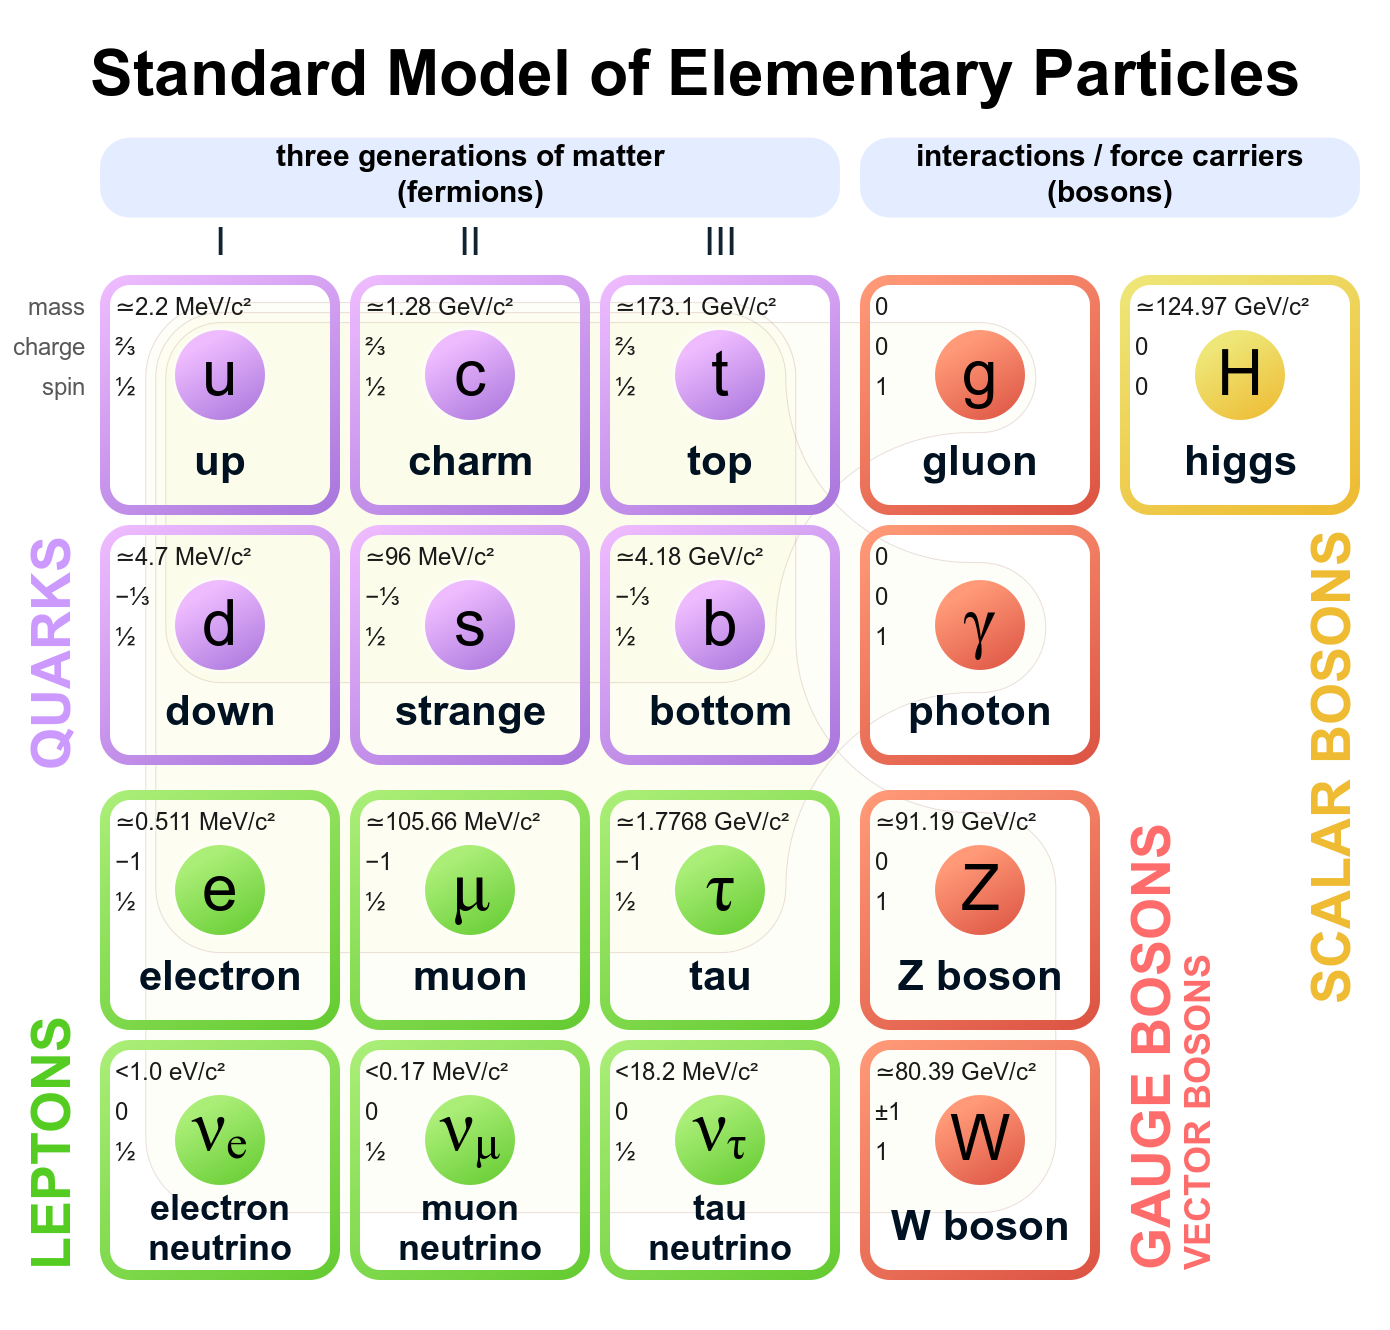
\includegraphics[width=0.65\textwidth]{fig/theory/Standard_Model_of_Elementary_Particles.png}
		\caption[Table of elementary particles in the SM. The leftmost three columns correspond to three generations of fermions, 
		the fourth column from the left shows the gauge bosons which mediate the elementary forces, and the rightmost column shows the Higgs boson. 
		For each particle, mass, charge, and spin are labeled, with mass values given as of 2019.]
		{Table~\cite{SMImage} of elementary particles in the SM. The leftmost three columns correspond to three generations of fermions, 
		the fourth column from the left shows the gauge bosons which mediate the fundamental forces, and the rightmost column shows the Higgs boson. 
		For each particle, mass, charge, and spin are labeled, with mass values given as of 2019.}
		\label{fig:SMParticles}
	\end{center}
\end{figure}

Figure \ref{fig:SMParticles} catalogs the elementary particles of the SM. These particles come in two broad types: fermions and bosons. Fermions are particles of half-integer spin that obey 
the Pauli exclusion principle. They are, therefore, responsible for the structure of matter. 
Each fermion has a corresponding antiparticle that has opposite electrical charge, but is otherwise identical. 
The fermions are subdivided into two types in three generations, the generations corresponding to mass.
Quarks are fermions that carry both fractional electric charge and color charge, so they participate in the electroweak and strong interactions. 
Leptons are fermions that carry integer electric charge and participate in the electroweak interaction.
In contrast to fermions, bosons have integer spin. The vector gauge bosons function as mediators of the fundamental forces of nature. 
The gluons mediate the strong force, the photon the electromagnetic force, and the W and Z bosons the weak force. 
Finally, the electrically neutral, scalar Higgs boson emerges due to electroweak symmetry breaking, described later in this section. The interaction of the Higgs 
with the other particles in the SM is responsible for particle masses. 
In the context of this thesis, which is a search for \hzg{}, the most relevant elementary particles are the Higgs boson, Z boson, leptons, and photon. 
Therefore, the remainder of this section will describe electroweak theory and the Higgs mechanism in more detail. Other aspects of the SM, such as quantum chromodynamics, 
are of importance in collider physics, but of less relevance for this specific search. Such topics are omitted in order to narrow the scope of the discussion.

\section{Electroweak Theory}
To motivate the Higgs mechanism and Higgs interactions, it is useful to first consider the electroweak interaction absent the Higgs. The electroweak piece of the 
SM Lagrangian can be written as 
\begin{align}
	& \mathcal{L}_{EW} = -\frac{1}{4}A_a^{\mu\nu}A^a_{\mu\nu} - \frac{1}{4}B^{\mu\nu}B_{\mu\nu} + i\sum_L \bar{L}\gamma^{\mu}D_{\mu,L}L + i\sum_R \bar{R}\gamma^{\mu}D_{\mu,R}R \label{eqn:LEWK}\\
	& A^a_{\mu\nu} = \partial_{\mu}A_{\nu}^{a} - \partial_{\nu}A_{\mu} + g\varepsilon_{abc}W^{b}_{\mu}W^{c}_{\nu} \\
	& B_{\mu\nu} = \partial_{\mu}B_{\nu} - \partial_{\nu}B_{\mu} \\
	& D_{\mu,L} = \partial_{\mu} + \frac{ig}{2}\tau\cdot A_{\mu} + \frac{ig'}{2}B_{\mu}Y \label{eqn:DL}\\
	& D_{\mu,R} = \partial_{\mu} + \frac{ig'}{2}B_{\mu}Y. \label{eqn:DR}
\end{align}
In the above equations, $A_{\mu\nu}^a$ represents an SU(2)$_L$ triplet of gauge fields and $B_{\mu\nu}$ represents a U(1) gauge field. The third and fourth terms in equation \ref{eqn:LEWK} 
describe the interactions of these gauge fields with the fermions, both quarks and leptons. Note that the interaction depends on the chirality of the fermions, where the left-handed 
fermions are denoted as $L$ and the right-handed as $R$. The right-handed fermions interact only with the U(1) field, while the left-handed fermions interact with the U(1) and SU(2)$_L$ fields. 
This is encoded by the derivative operators $D_{\mu,L}$ and $D_{\mu,R}$ defined in equations \ref{eqn:DL} and \ref{eqn:DR} in terms of the fields, Pauli matrices ($\tau$), hypercharge operator Y, and the couplings $g$ and $g'$. 

\section{Spontaneous Symmetry Breaking (Higgs Mechanism)}
One important property of the electroweak Lagrangian in equation \ref{eqn:LEWK} is that the bosons associated with the gauge fields are all massless. 
However, the direct observation of charged and neutral 
current interactions \cite{HASERT1973121,HASERT1973138} at CERN in 1973 implied that the W and Z boson must have relatively large masses in the range of 50--100\GeV. Indeed, the massive W and Z bosons were later discovered and measured \cite{UA1:1983crd,UA2:1983tsx} at the CERN Super Proton Synchroton in 1983. 
A solution to this shortcoming of the electroweak theory came in the form of the Higgs mechanism \cite{Englert:1964et,Higgs:1964ia,Higgs:1964pj},
which spontaneously breaks the SU(2)xU(1) gauge symmetry. One consequence of this is the addition of a real 
Higgs field accompanied by a massive Higgs boson. The W and Z boson masses arise naturally due to the electroweak symmetry breaking, 
while fermion masses are explained via additional Yukawa couplings to the Higgs boson. 
The discovery of the Higgs boson and subsequent measurements of its properties have provided experimental verification that the Higgs mechanism 
is a central piece of the Standard Model. 

To understand how the Higgs mechanism works, consider the introduction of a complex scalar field $\sf \Phi$, which 
transforms as a doublet under SU(2)$_L$.
\begin{equation}
    \label{eqn:higgsField}
    \Phi = 
    \begin{bmatrix}
        \phi^{+} \\ 
        \phi^{0}
    \end{bmatrix}
\end{equation}
Its contribution to the Lagrangian is given by:
\begin{equation}
    \mathcal{L_{H}} = (D^{\mu}_L\Phi)^{\dagger}(D_{\mu,L}\Phi) - V(\Phi)
    \label{LHiggs}
\end{equation}
where the Higgs potential takes the form
\begin{equation}
    V(\Phi) = \mu^{2}|\Phi^{\dagger}\Phi| + \lambda \Big(|\Phi^{\dagger}\Phi|\Big)^{2}.
    \label{VHiggs}
\end{equation}
Consider the case in which the parameters of the Higgs potential $\lambda$ and $\mu$ satisfy the conditions 
$\lambda > 0$ and $\mu^{2} < 0$. Then the shape of the potential is shown in Fig. \ref{fig:VHiggs} (right). There is no minimum of the 
potential at $\Phi = 0$. Rather, an infinite set of minima lie around a circle in the complex plane. Hence, it is said that $\Phi$ 
has a nonzero vacuum expectation value (VEV). The value of the VEV in terms of $\mu$ and $\lambda$ can be determined by explicitly
minimizing the potential:
\begin{align*}
    \frac{\partial}{\partial(\Phi^{\dagger}\Phi)}V(\Phi) &= 0 \\
    \mu^{2} + 2\lambda\Big(|\Phi^{\dagger}\Phi|\Big) &= 0 \\
    \mu^{2} + 2\lambda\Big[(\phi^{+})^{2} + (\phi^{0})^{2}\Big] &= 0 \numberthis
    \label{VHiggsMinimization}
\end{align*}
This can be minimized in many ways depending on individual values of $\phi^{+}$ and $\phi^{0}$ in the vacuum. By convention,
and without loss of generality, we choose the case in which $\phi^{+} = 0$. In this case we obtain the equation
\begin{equation}
    \phi^{0} = \sqrt{\frac{-\mu^{2}}{2\lambda}} = \frac{1}{\sqrt{2}}v
\end{equation}
where we have defined $v \equiv \sqrt{-\mu^{2}/\lambda}$.

\begin{figure}
	\begin{center}
	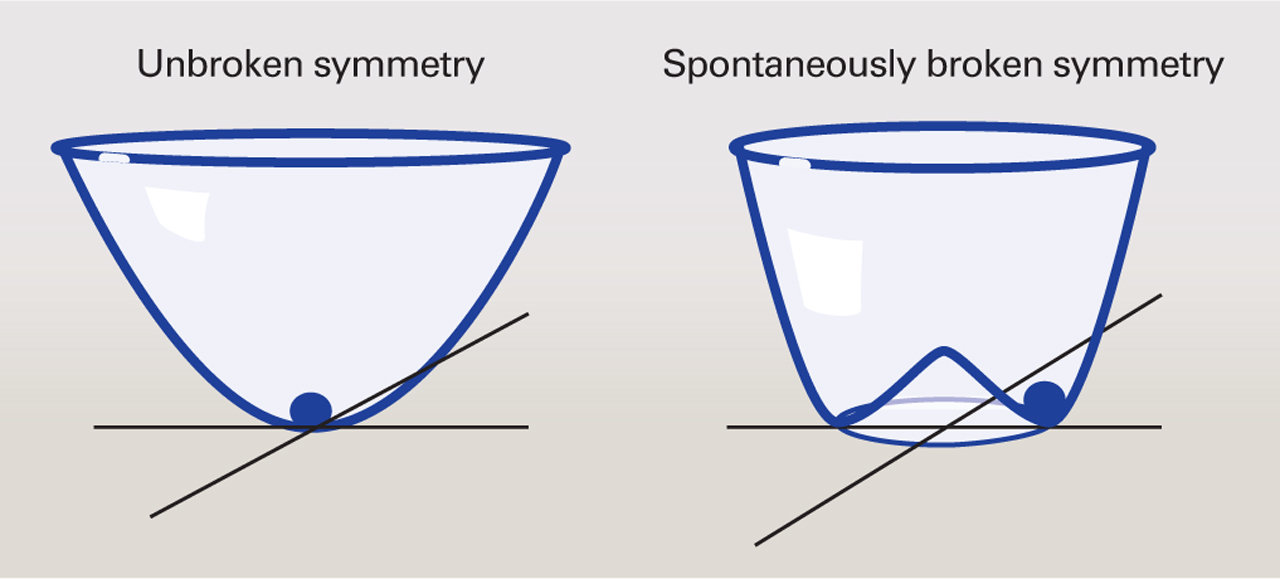
\includegraphics[width=0.75\textwidth]{fig/theory/spont_sym_breaking.jpg}
		\caption
		[Comparison of the shapes of complex scalar potentials without symmetry breaking (left) and with spontaneous symmetry breaking (right). 
		The transverse axes represent the real-imaginary $\Phi$ plane, 
		and the vertical axis represents the magnitude of the potential $V(\Phi)$. The diagram at right corresponds to the shape of the Higgs potential in the SM.]
		{Comparison of the shapes of complex scalar potentials without symmetry breaking (left) and with spontaneous symmetry breaking (right)~\cite{VHiggsImage}. 
		The transverse axes represent the real-imaginary $\Phi$ plane, 
		and the vertical axis represents the magnitude of the potential $V(\Phi)$. The diagram at right corresponds to the shape of the Higgs potential in the SM.}
		\label{fig:VHiggs}
	\end{center}
\end{figure}

The existence of the Higgs VEV has profound implications. To see this, it is helpful to reparameterize the scalar doublet field
$\Phi$ as follows:
\begin{equation}
    \Phi = \frac{1}{\sqrt{2}}e^{i\frac{\tau^{a}}{2}\theta_{a}(x)}
    \begin{bmatrix}
        0 \\
        v + h(x)
    \end{bmatrix}
    \label{reparamHiggsField}
\end{equation}
As $\Phi$ is invariant under local SU(2)$_L$ gauge transformations, the prefactor may be rotated away. This is equivalent to setting 
$\theta(x) = 0$ in equation \ref{reparamHiggsField}. This choice of gauge is known as the unitary gauge, and leads to 
\begin{equation}
    \Phi = \frac{1}{\sqrt{2}}
    \begin{bmatrix}
        0 \\
        v + h(x)
    \end{bmatrix}
    \label{HiggsFieldUnitaryGauge}
\end{equation}
Given the above form of $\Phi$, we can now evaluate the Higgs Lagrangian (equation \ref{LHiggs}), starting with the kinetic term
$(D^{\mu}_L\Phi)^{\dagger}(D_{\mu,L}\Phi)$.
\begin{align*}
    (D^{\mu}_L\Phi)^{\dagger}(D_{\mu,L}\Phi) &= \Big| (\partial_{\mu} - \frac{ig}{2}\tau\cdot A_{\mu} - \frac{ig'}{2}B_{\mu}Y)\Phi\Big|^{2} \\
    &= \frac{1}{2}
    \Big| 
    \begin{bmatrix}
        \partial_{\mu} - \frac{i}{2}(gA_{\mu}^{3} + g'B_{\mu}) & -\frac{ig}{2}(A_{\mu}^{1} - iA_{\mu}^{2}) \\
            -\frac{ig}{2}(A_{\mu}^{1} + iA_{\mu}^{2}) & \partial_{\mu} + \frac{i}{2}(gA_{\mu}^{3} - g'B_{\mu})
    \end{bmatrix} 
    \begin{bmatrix}
        0 \\ 
        v + h(x)
    \end{bmatrix} 
    \Big|^{2} \\ &=  
    \frac{1}{2}\Big| 
    \begin{bmatrix}
        -\frac{ig}{2}(A_{\mu}^{1} - iA_{\mu}^{2})(v + h(x)) \\
        \partial_{\mu}h(x) + \frac{i}{2}(gA_{\mu}^{3} - g'B_{\mu})(v + h(x))
    \end{bmatrix}
    \Big|^{2} \\ &= 
    \frac{1}{2}\partial_{\mu}h(x)\partial^{\mu}h(x) + \frac{1}{8}(gA_{\mu}^{3} - g'B_{\mu})(gA^{\mu}_{3} - g'B^{\mu})(v + h(x))^{2} \\ &+ 
    \frac{g^{2}}{8}(A_{\mu}^{1} - iA_{\mu}^{2})(A_{\mu}^{1} + iA_{\mu}^{2})(v + h(x))^{2} \label{kinHiggsExpansion} \numberthis 
\end{align*}
With some foreknowledge of the result, we define the physical gauge fields and their masses.
\begin{align}
    W_{\mu}^{\pm} &= \frac{1}{\sqrt{2}}(A_{\mu}^{1} \mp iA_{\mu}^{2}) \; &m_{W} = \frac{gv}{2} \\
    Z_{\mu} &= \frac{1}{\sqrt{g^{2} + g'^{2}}}(gA_{\mu}^{3} - g'B_{\mu}) \; &m_{Z} = \sqrt{g^{2} + g'^{2}}\frac{v}{2} \\
    A_{\mu} &= \frac{1}{\sqrt{g^{2} + g'^{2}}}(g'A_{\mu}^{3} + gB_{\mu}) \; &m_{A} = 0
    \label{gaugeBosonsAndMasses}
\end{align}
Then the kinetic term of the Higgs Lagrangian can be recast as
\begin{align*}
    (D^{\mu}_L\Phi)^{\dagger}(D_{\mu,L}\Phi) &= \frac{1}{2}\partial_{\mu}h(x)\partial^{\mu}h(x) \\ 
    &+ \frac{1}{2}m_{Z}^{2}Z_{\mu}Z^{\mu} + m_{W}^{2}W_{\mu}^{+}W^{-\mu} \\
    &+ \frac{v}{4}(g^{2} + g'^{2})Z_{\mu}Z^{\mu}h + \frac{1}{8}(g^{2} + g'^{2})Z_{\mu}Z^{\mu}h^{2} \\
    &+ \frac{v}{4}g^{2}W_{\mu}^{+}W^{-\mu}h + \frac{1}{8}g^{2}W_{\mu}^{+}W^{-\mu}h^{2} \label{kinHiggsMasses}\numberthis
\end{align*}
Equation \ref{kinHiggsMasses} provides a great deal of information on the physical ramifications of the Higgs mechanism.
The first term is the kinetic term of the physical Higgs boson field. The second and third terms are the mass terms of the Z and W 
bosons, respectively. The fourth and fifth terms show the linear and quadratic couplings of the Z boson to the Higgs boson, respectively.
Finally, the sixth and seventh terms show the linear and quadratic couplings of the W boson to the Higgs boson, respectively. 
Given the form of equation \ref{HiggsFieldUnitaryGauge}, a similar expansion can be carried out on the Higgs potential
(equation \ref{VHiggs}). Here, the terms involving the physical Higgs boson are most interesting, so constant terms are dropped.
\begin{align*}
    V(\Phi) &= \frac{\mu^{2}}{2}(v+h)^{2} + \frac{\lambda}{4}((v+h)^{2})^{2} \\
    &\rightarrow \lambda v^{2}h^{2} + \lambda vh^{3} + \frac{\lambda}{4}h^{4} \label{expandedVHiggs} \numberthis
\end{align*}
The first term is a Higgs mass term, with $m_{H} = \sqrt{2\lambda v^{2}}$. The second and third terms describe the Higgs 
trilinear and quartic self-couplings, respectively.

The Lagrangian including the Higgs doublet $\Phi$ can be further extended to incorporate interactions between the Higgs and fermion fields. These interactions, along with the nonzero Higgs VEV, provide a mechanism to generate the fermion masses. The interactions take the 
form of Yukawa couplings:
\begin{equation}
    \mathcal{L}_{Yukawa} = Y_{ij}^{d}\bar{Q}^{i}_{L}\Phi d_{R}^{j} + Y_{ij}^{u}\bar{Q}^{i}_{L}\tilde{\Phi} u_{R}^{j} 
    + Y_{ij}^{e}\bar{L}^{i}_{L}\Phi e_{R}^{j} + h.c.,
    \label{LYukawa}
\end{equation}
where $\tilde{\Phi} \equiv i\tau_{2}\Phi^{*}$, and $u$, $d$, and $e$ represent up-type quarks, down-type quarks, and leptons, respectively. The constants $Y_{ij}^a$ denote the Yukawa couplings in each case, $Q^i$ is the set of SU(2) quark doublets, and $L^i$ is the set of SU(2) lepton doublets.
\begin{equation}
    \tilde{\Phi} \equiv i\tau_{2}\Phi^{*}
    \label{PhiDual}
\end{equation}
Plugging in the unitary gauge parameterization of equation \ref{HiggsFieldUnitaryGauge}, this evaluates to 
\begin{align}
    \mathcal{L}_{Yukawa} = \frac{Y_{ij}^{d}}{\sqrt{2}}\bar{d}_{L}^{i}(v + h)d_{R}^{j} 
    + \frac{Y_{ij}^{u}}{\sqrt{2}}\bar{u}_{L}^{i}(v+h)u_{R}^{j} + \frac{Y_{ij}^{e}}{\sqrt{2}}\bar{e}_{L}^{i}(v+h)e_{R}^{j}
    \label{expandedLYuk}
\end{align}
It is worth looking closely at the terms in equation \ref{expandedLYuk}. For a given fermion type, the first term in the parentheses
is a fermion mass term. The second term in the parentheses gives the coupling of the fermion to the Higgs boson. With this in mind, 
we observe that the fermion mass is given in terms of the couplings and the Higgs vev by 
\begin{equation}
    m_{f} = \frac{y_{f}v}{\sqrt{2}}
    \label{fermionMass}
\end{equation}
where $y_{f}$ is the relevant value taken from the Yukawa coupling matrix. In addition, we see that the strength of the fermion coupling
to the Higgs boson is given by $\frac{m_{f}}{v}$. Thus, fermions couple to the Higgs boson with strength directly proportional 
to their masses. This result has important consequences in the context of collider experiments, as it regulates the rates of
Higgs production and decay related to each fermion-Higgs interaction. 

%The existence of the Higgs VEV leads naturally to the masses of the W and Z bosons. This can be shown by squaring the covariant 
%derivative acting on the scalar doublet $\Phi$ and evaluating the result in the vacuum. Note that in the vacuum, all terms involving 
%the partial derivative $\partial_{\mu}$ will yield zero contribution. Therefore, keeping only the relevant terms, the squared covariant 
%derivative reduces to
%\begin{equation}
%    |D_{\mu}|^{2} \rightarrow (\frac{g}{2}A_{\mu}^{a}\tau^{a} +\frac{g'}{2}B_{\mu})(\frac{g}{2}A^{b\mu}\tau^{b} + \frac{g'}{2}B^{\mu})
%    \label{covDerivSquared}
%\end{equation}
%Evaluating this in the vacuum yields
%\begin{align}
%    \Delta\mathcal{L} &= \frac{1}{2}
%    \begin{bmatrix}0 & v
%    \end{bmatrix}
%    (\frac{g}{2}A_{\mu}^{a}\tau^{a} +\frac{g'}{2}B_{\mu})(\frac{g}{2}A^{b\mu}\tau^{b} + \frac{g'}{2}B^{\mu}) 
%    \begin{bmatrix}
%        0 \\ 
%        v
%    \end{bmatrix} \\ 
%    \Delta\mathcal{L} &=
%    \frac{1}{2}\frac{v^{2}}{4}[g^{2}(A_{\mu}^{1})^{2} g^{2}(A_{\mu}^{2})^{2} + (g'B_{\mu} - gA_{\mu}^{3})^{2}]
%\end{align}
%From this, we can identify the fields and masses for the positively and negatively charged W bosons and the neutral Z boson and photon. 
%These are as follows:


\section{Higgs Production}

At a hadron collider like the LHC, the Higgs boson can be produced via several different mechanisms, each mechanism occuring at a certain rate. The dominant production 
mechanism is gluon-gluon fusion (ggH), followed by vector boson fusion (VBF) production, which is about an order of magnitude rarer. Less common production mechanisms, but 
still relevant for a search at the LHC, are the associated production mechanisms WH, ZH, and t$\bar{t}$H. The cross sections for each Higgs production mechanism as a function of 
center of mass energy are shown in Fig. \ref{fig:higgs_prod}.

\begin{figure}
	\begin{center}
	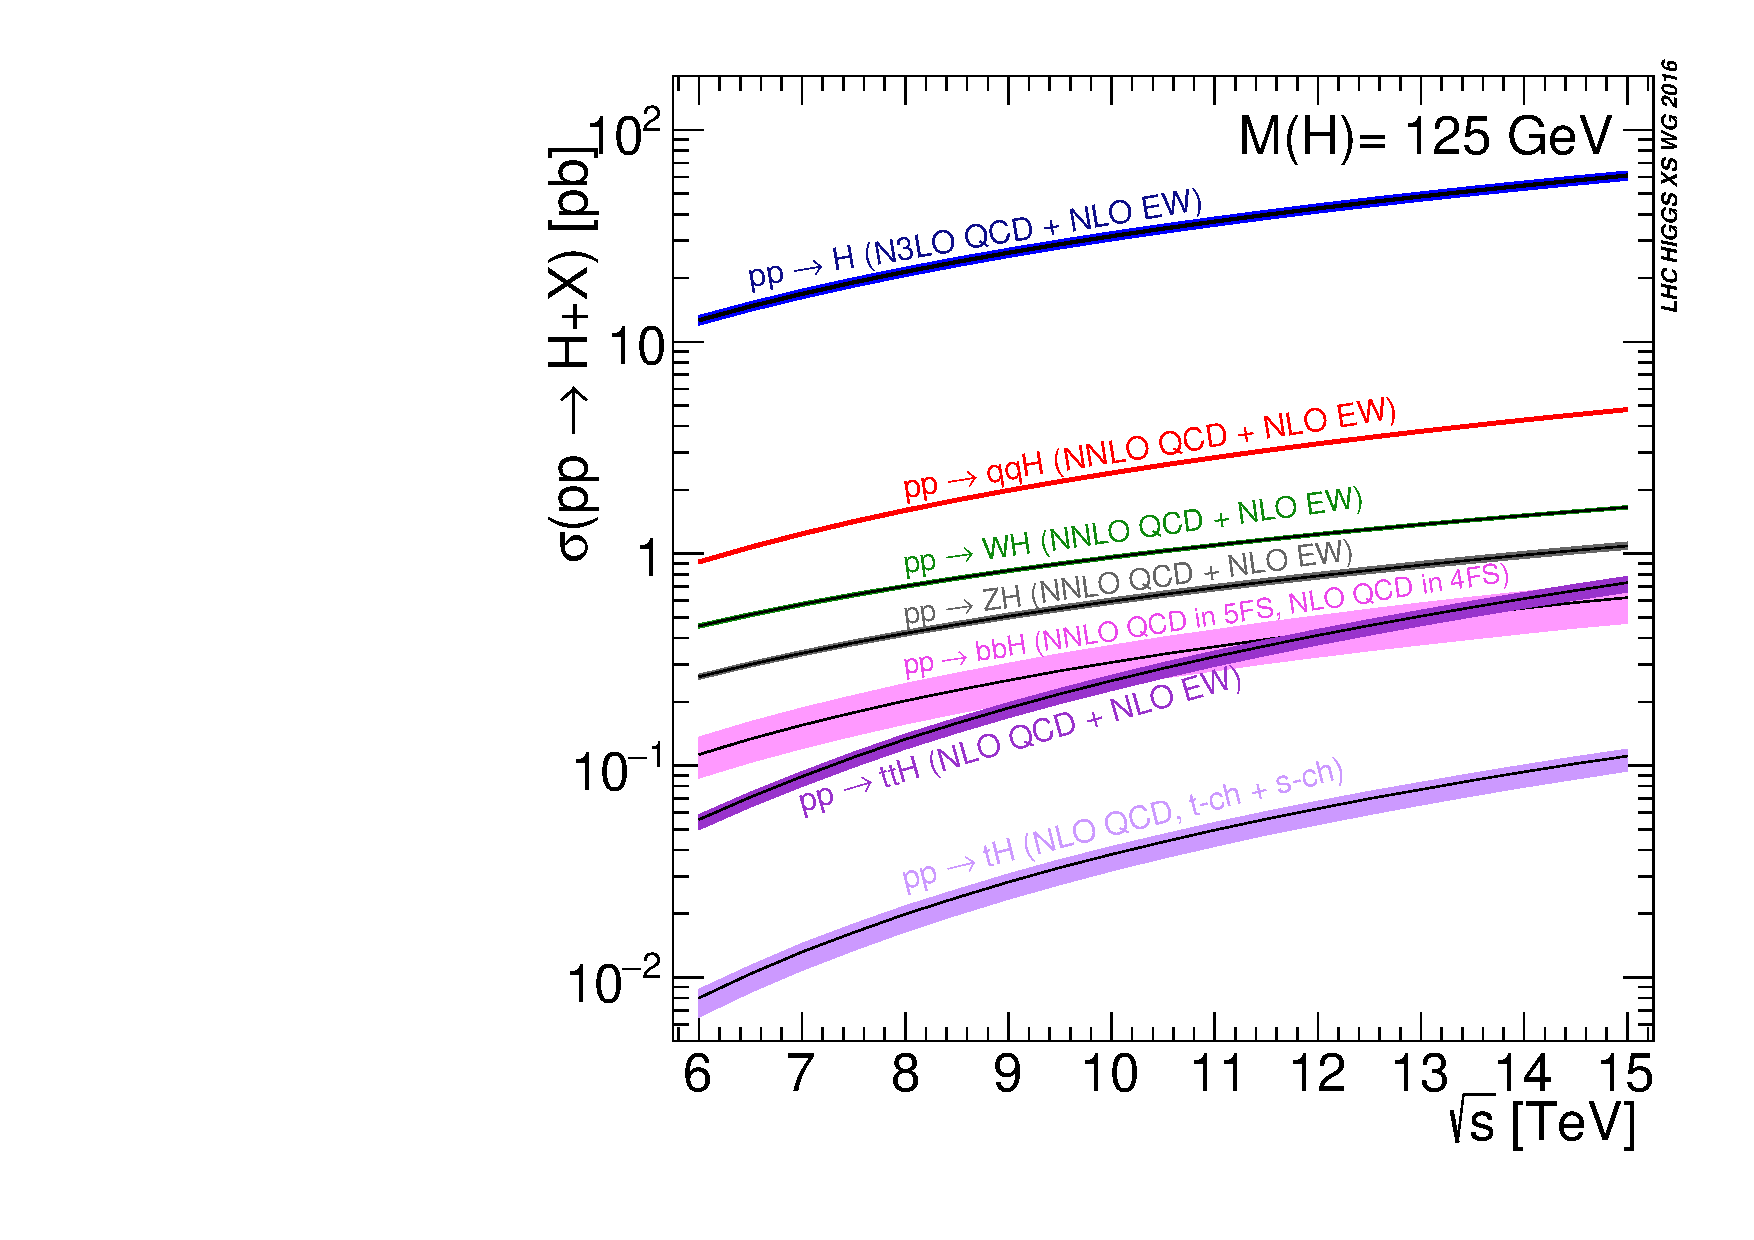
\includegraphics[width=0.75\textwidth]{fig/theory/Plot_Escan_H125_new_sqrt.pdf}
	\caption{Cross sections for different Higgs boson production mechanisms as a function of center of mass energy.}
	\label{fig:higgs_prod}
	\end{center}
\end{figure}

\section{Higgs Decay}

The Higgs boson decays rapidly after it is produced at the LHC. It can decay into a variety of final states, each occuring at a certain rate. Tree-level Higgs decays occur at rates 
proportional to the square of the mass of the decay products. Decays to b$\bar{b}$, WW, $\tau^+\tau^-$, and ZZ, are among the most common and experimentally accessible at the LHC. Other Higgs decays 
occur at loop-level, including $\PH \to \Pg\Pg$ and \hzg. Figure \ref{fig:higgs_br} shows the branching fractions at $\sqrt{s}=13$\TeV for different decay channels as a function of Higgs boson mass. 
We see that the branching fraction of \hzg is suppressed relative to several other production modes, so a search for \hzg must rely on the clean $\ell^+\ell^-\gamma$ signature.

\begin{figure}
	\begin{center}
	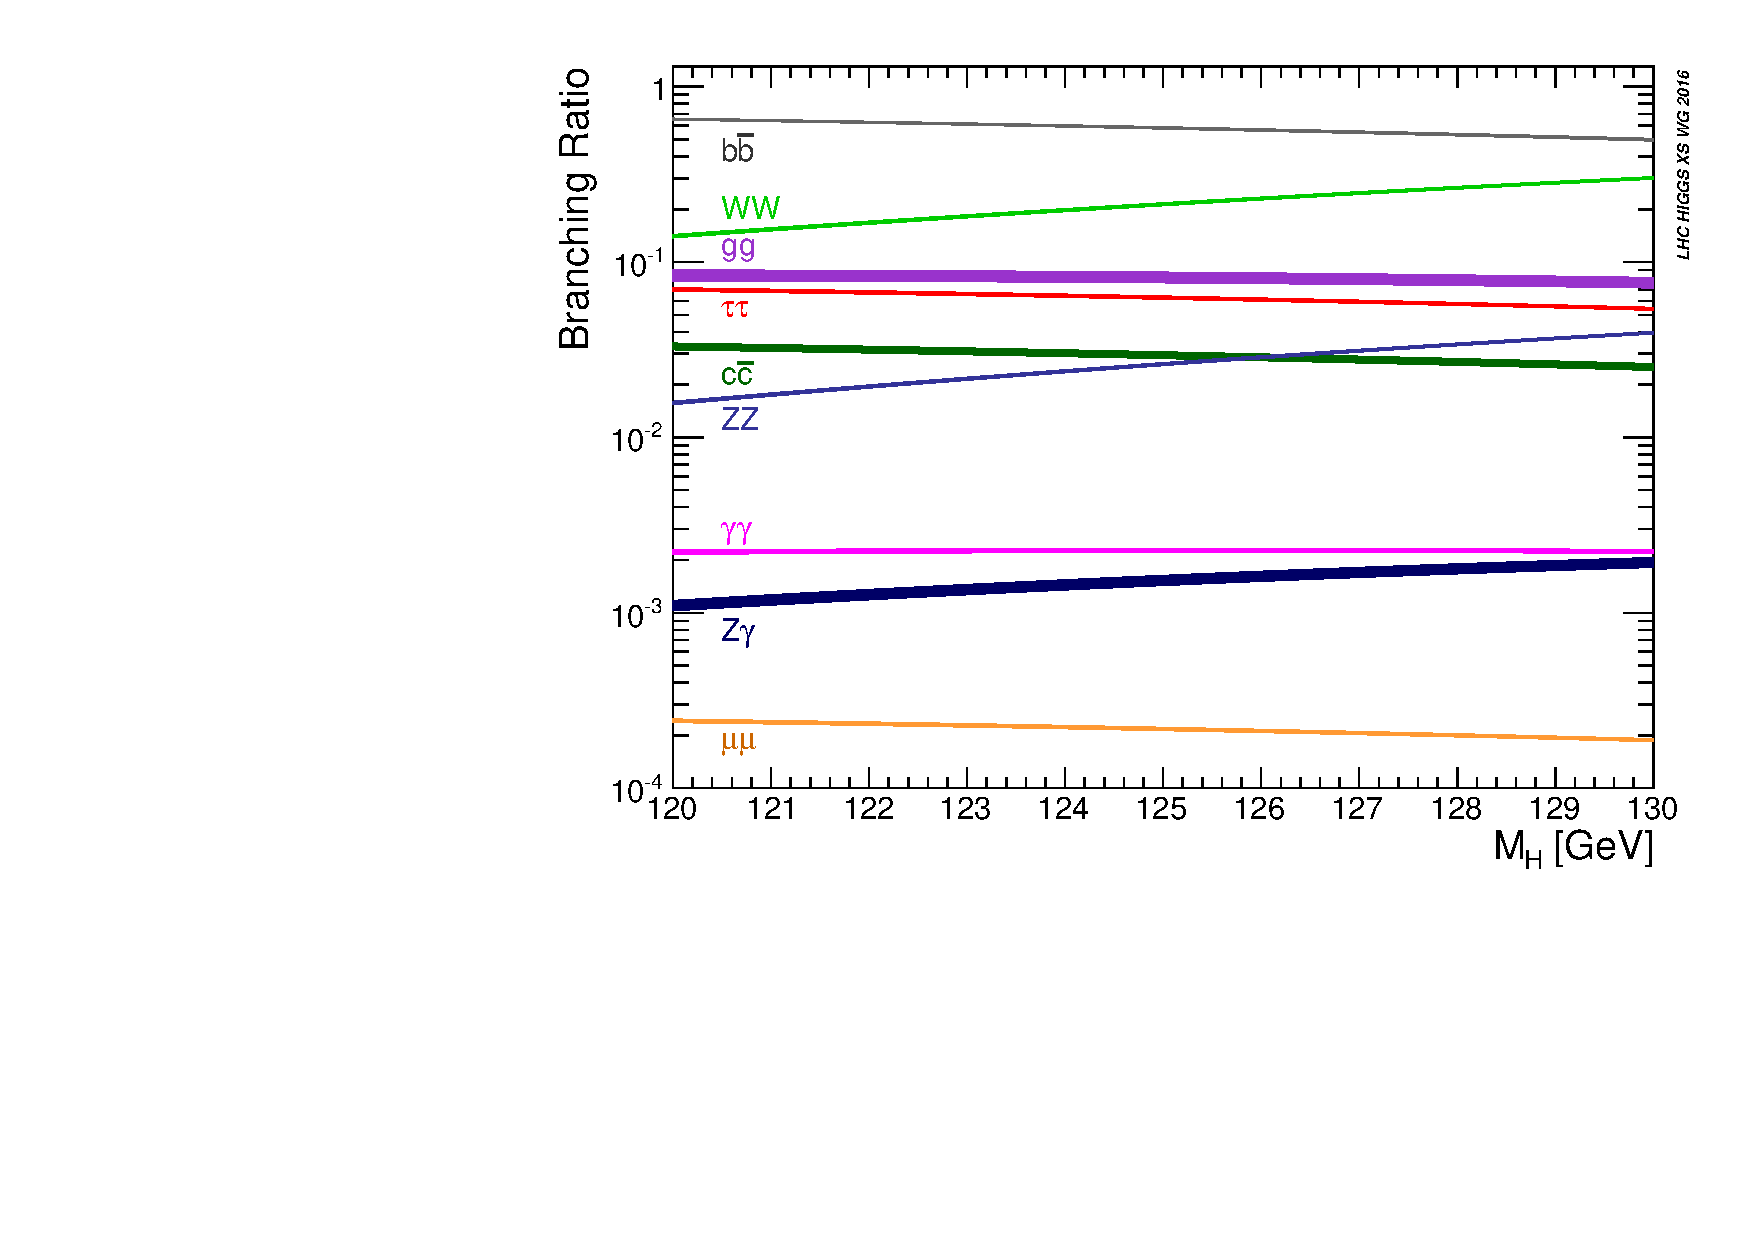
\includegraphics[width=0.75\textwidth]{fig/theory/SMHiggsBR.YR4-rect.pdf}
		\caption{Branching fraction of \hzg decay as a function of Higgs boson mass.}
		\label{fig:higgs_br}
	\end{center}
\end{figure}

\section{Physics Beyond the Standard Model}

One of the goals of the LHC is to search for BSM physics. While the decay \hzg{} is predicted in the SM, searching for it and measuring its branching fraction can indirectly probe potential 
new physics phenomena. A few unique features of \hzg{} make it well-suited as a BSM probe. First, the decay is loop-induced, which means that the introduction of new particles will contribute 
to the loop, interfering and altering the final branching fraction. Secondly, the decay \hgg{} is a very similar loop-induced process that has been discovered and measured extensively 
by the CMS and ATLAS Collaborations [REFS]. This means any new particle content entering into the \hzg{} loop will also enter into the \hgg{} loop. However, in the case of \hzg{}, the
Z boson couples to loop particles according to the SU(2)xU(1) quantum number rather than just the electric charge, as is the case for \hgg{}. 
It follows that potential BSM physics scenarios can shift the 
branching fractions of \hzg{} and \hgg{} by differing amounts, making the ratio $\mathcal{B}(\PH\rightarrow\PZ\gamma)/\mathcal{B}(\PH\rightarrow\gamma\gamma)$ a sensitive observable. In the SM, 
$\mathcal{B}(\PH\rightarrow\PZ\gamma)/\mathcal{B}(\PH\rightarrow\gamma\gamma) = 0.69 \pm 0.04$. A measurement of a significant deviation from this value would be an indicator of possible BSM physics.
Below, we describe a few examples of BSM scenarios that can affect this ratio.

One way to consider BSM effects in the context of \hzg{} is to introduce new particles, like a W' boson, charged scalar, or a pair of charged leptons. 
This is the approach taken by Carena, Low, and Wagner~\cite{Zg_theory_decaywidth}. The W' possibility is motivated by the fact that the W boson loop is the dominant 
contribution in the SM. The W' can be defined by an SU(2) triplet and characterized by mass and Higgs coupling parameters. Figure \ref{fig:rzg_bsm} (left) shows contours of constant branching fraction 
enhancement in the \hzg{} and \hgg{} decay channels in the mass-coupling plane for the W' model. 
Depending on the parameter values, the level of enhancement can be up to double the SM value, and it differs 
significantly in the two channels. Similarly, we can imagine a new charged scalar or a pair of new charged leptons. The branching fraction enhancement contour plots in Fig. \ref{fig:rzg_bsm} show that for similar regions in the mass-coupling plane, \hzg{} can be enhanced, while \hgg{} is simultaneously diminished. 

Other relevant BSM physics models include extended Higgs sectors. Such models often contain charged Higgs bosons, which enter into the \hzg{} and \hgg{} loops and impact the branching fractions. 
In Ref. \cite{Zg_theory_extension}, Chiang and Yagyu catalog extended Higgs models of varying types: models with one singly-charged boson, those with one singly-charged and one doubly-charged boson, 
and those with two singly-charged bosons. In total, the authors consider thirteen models, including the two Higgs doublet model, the minimal SUSY model, and the Higgs triplet model. 
Figure \ref{fig:exthiggs} gives the ratio of decay widths $\Gamma(\PH\rightarrow\PZ\gamma)/\Gamma(\PH\rightarrow\gamma\gamma)$ as a function of the mass coefficient of the additional scalar field(s) for seven of the models. It is evident that, for mass scales accessible at the LHC, the ratio can be significantly shifted relative to the SM expectation. 


\begin{figure}[tb]
	\begin{center}
		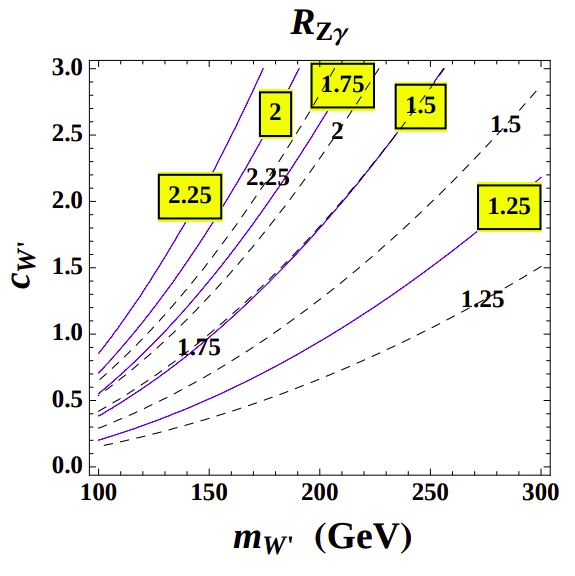
\includegraphics[width=0.30\textwidth, height=.30\textwidth]{fig/theory/rzgamma_wprime.png}
		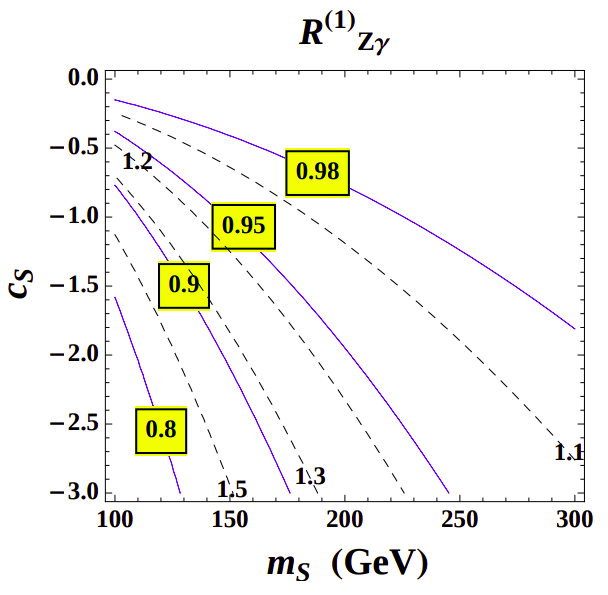
\includegraphics[width=0.30\textwidth, height=.30\textwidth]{fig/theory/rzgamma_scalar.png}
		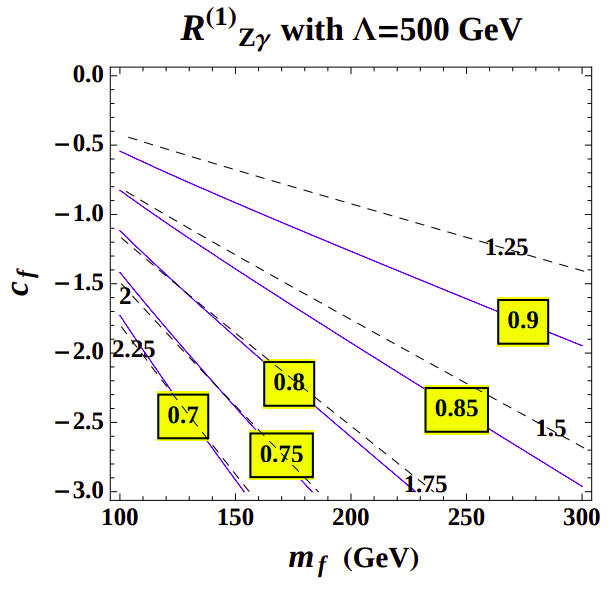
\includegraphics[width=0.30\textwidth, height=.30\textwidth]{fig/theory/rzgamma_fermion.png}
		\caption[Contours of constant branching fraction enhancement relative to the SM for the W' (left), charged scalar (center), 
		and charged lepton (right) scenarios. 
		The solid lines represent contours of enhancement in $\mathcal{B}$(\hzg), while the dashed lines correspond to \hgg{}. The yellow boxed numbers label the enhancement for each 
		\hzg{} contour, and the unboxed numbers label the enhancement for each \hgg{} contour.]
		{Contours of constant branching fraction enhancement relative to the SM for the W' (left), charged scalar (center), 
		and charged lepton (right) scenarios~\cite{Zg_theory_decaywidth}. 
		The solid lines represent contours of enhancement in $\mathcal{B}$(\hzg), while the dashed lines correspond to \hgg{}. The yellow boxed numbers label the enhancement for each 
		\hzg{} contour, and the unboxed numbers label the enhancement for each \hgg{} contour.}
		\label{fig:rzg_bsm}
	\end{center}
\end{figure}

\begin{figure}[tb]
	\begin{center}
		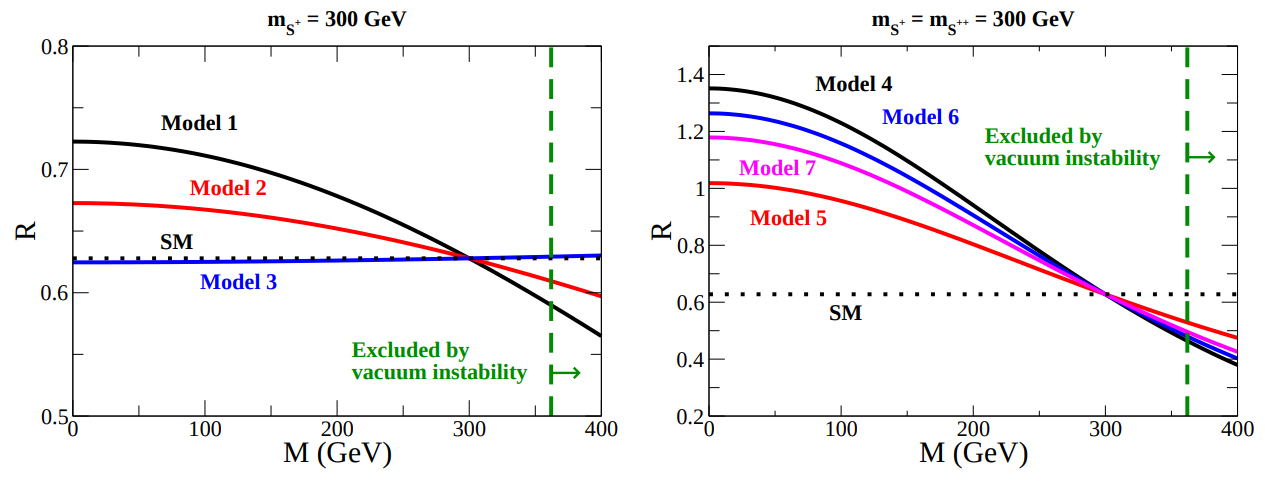
\includegraphics[width=0.9\textwidth]{fig/theory/rzgamma_exthiggs.png}
		\caption[Ratio of decay widths $\Gamma(\PH\rightarrow\PZ\gamma)/\Gamma(\PH\rightarrow\gamma\gamma)$ as a function of the mass coefficient of the additional scalar field(s) for 
		seven BSM models with extended Higgs sectors. 
		The models plotted on the left correspond to one additional singly-charged boson, and those on the right to one additional singly-charged and one additional doubly-charged boson.]
		{Ratio of decay widths $\Gamma(\PH\rightarrow\PZ\gamma)/\Gamma(\PH\rightarrow\gamma\gamma)$ as a function of the mass coefficient of the additional scalar field(s) for 
		seven BSM models with extended Higgs sectors~\cite{Zg_theory_extension}. 
		The models plotted on the left correspond to one additional singly-charged boson, and those on the right to one additional singly-charged and one additional doubly-charged boson.}
		\label{fig:exthiggs}
	\end{center}
\end{figure}


\chapter{Results and Interpretation}\label{sec:results}

Figures~\ref{fig:3} and \ref{fig:4} show the $m_{\ell^+\ell^-\gamma}$ distributions of the data events in each category.
The expected SM $\PH\to\PZ\gamma$ distributions, scaled by a factor of 10, are also shown.
Figure~\ref{fig:SignalBackground} shows the signal-plus-background fit to the data and the corresponding distribution after background subtraction for the sum of all categories. 
Each category is weighted by the factor $S/(S+B)$, where $S$ is the signal yield  
and $B$ is the background yield in the narrowest mass interval containing 95\% of the signal distribution.

\begin{figure}
  \centering
  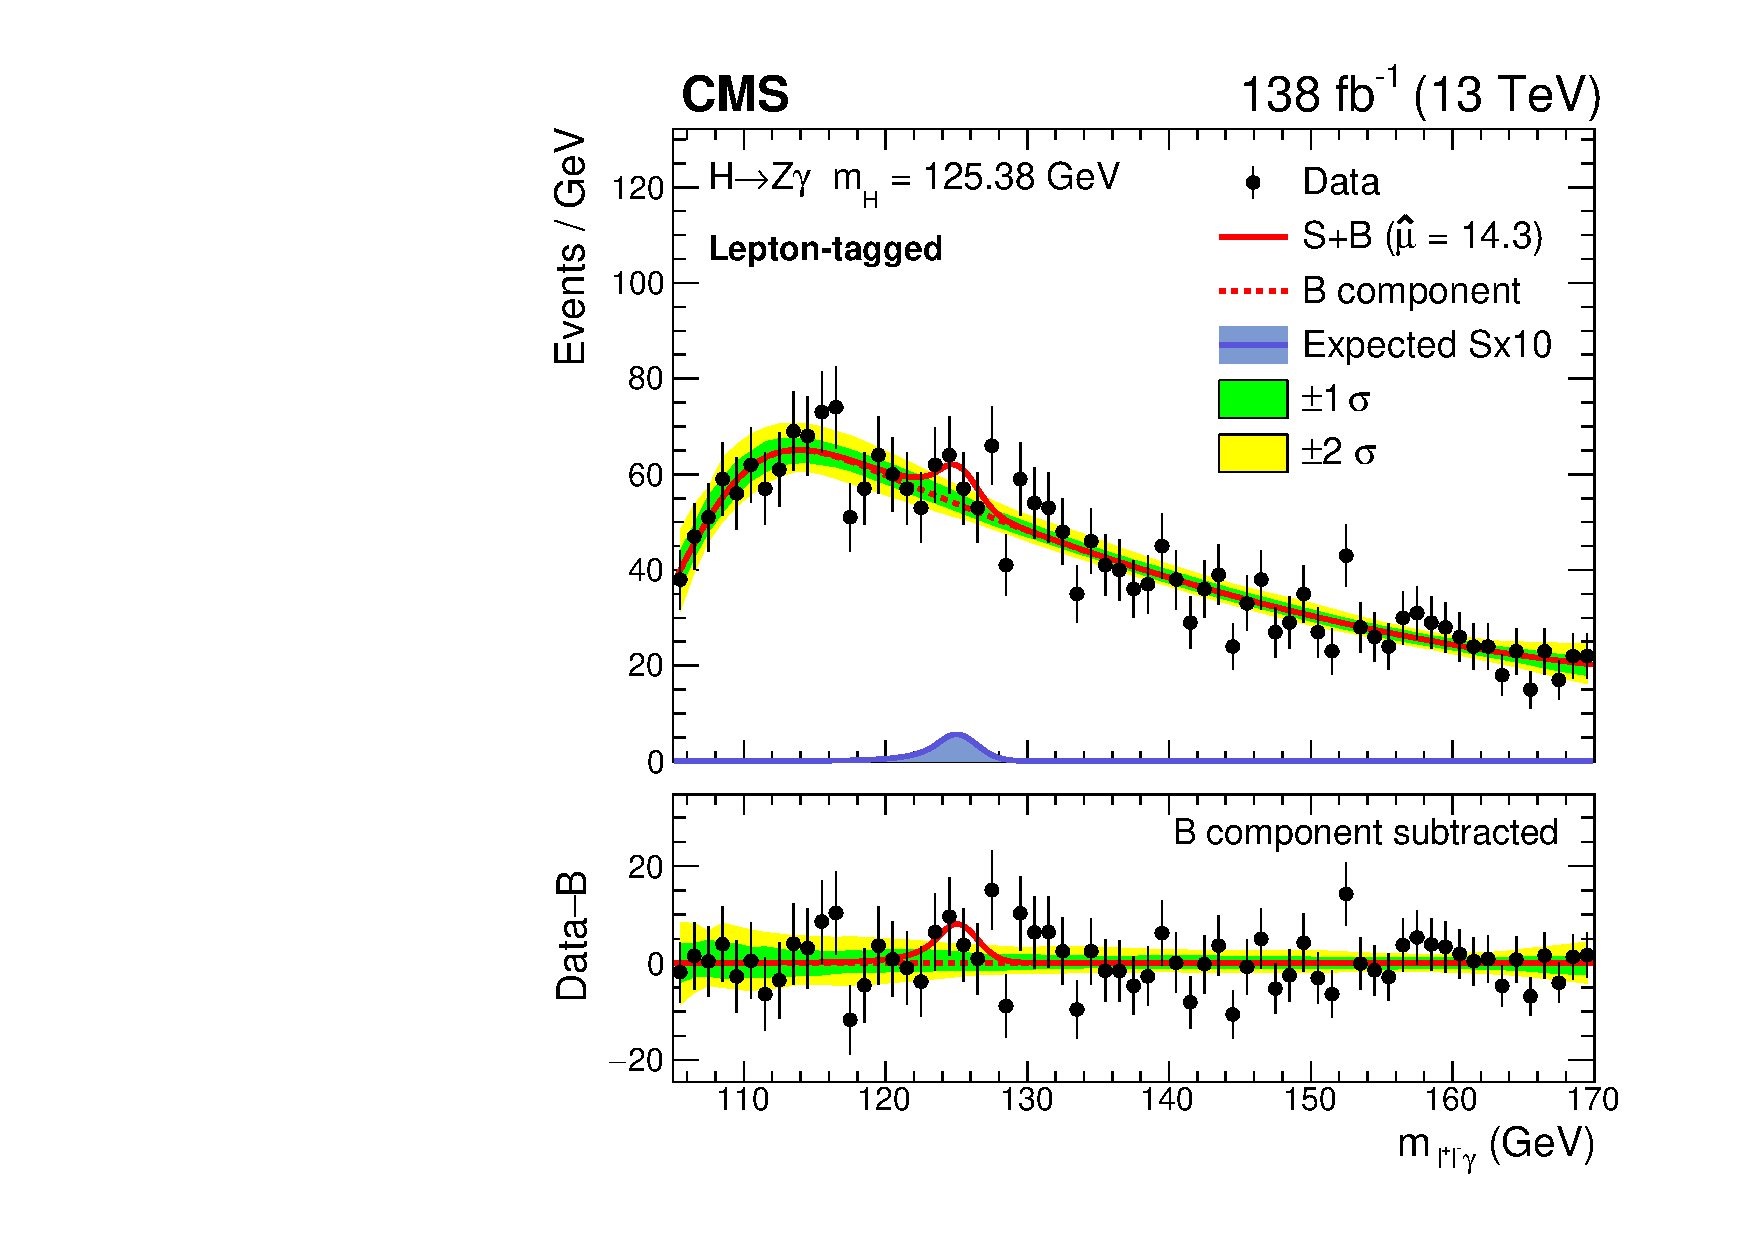
\includegraphics[width=0.45\textwidth]{fig/results/Figure_008.pdf}
  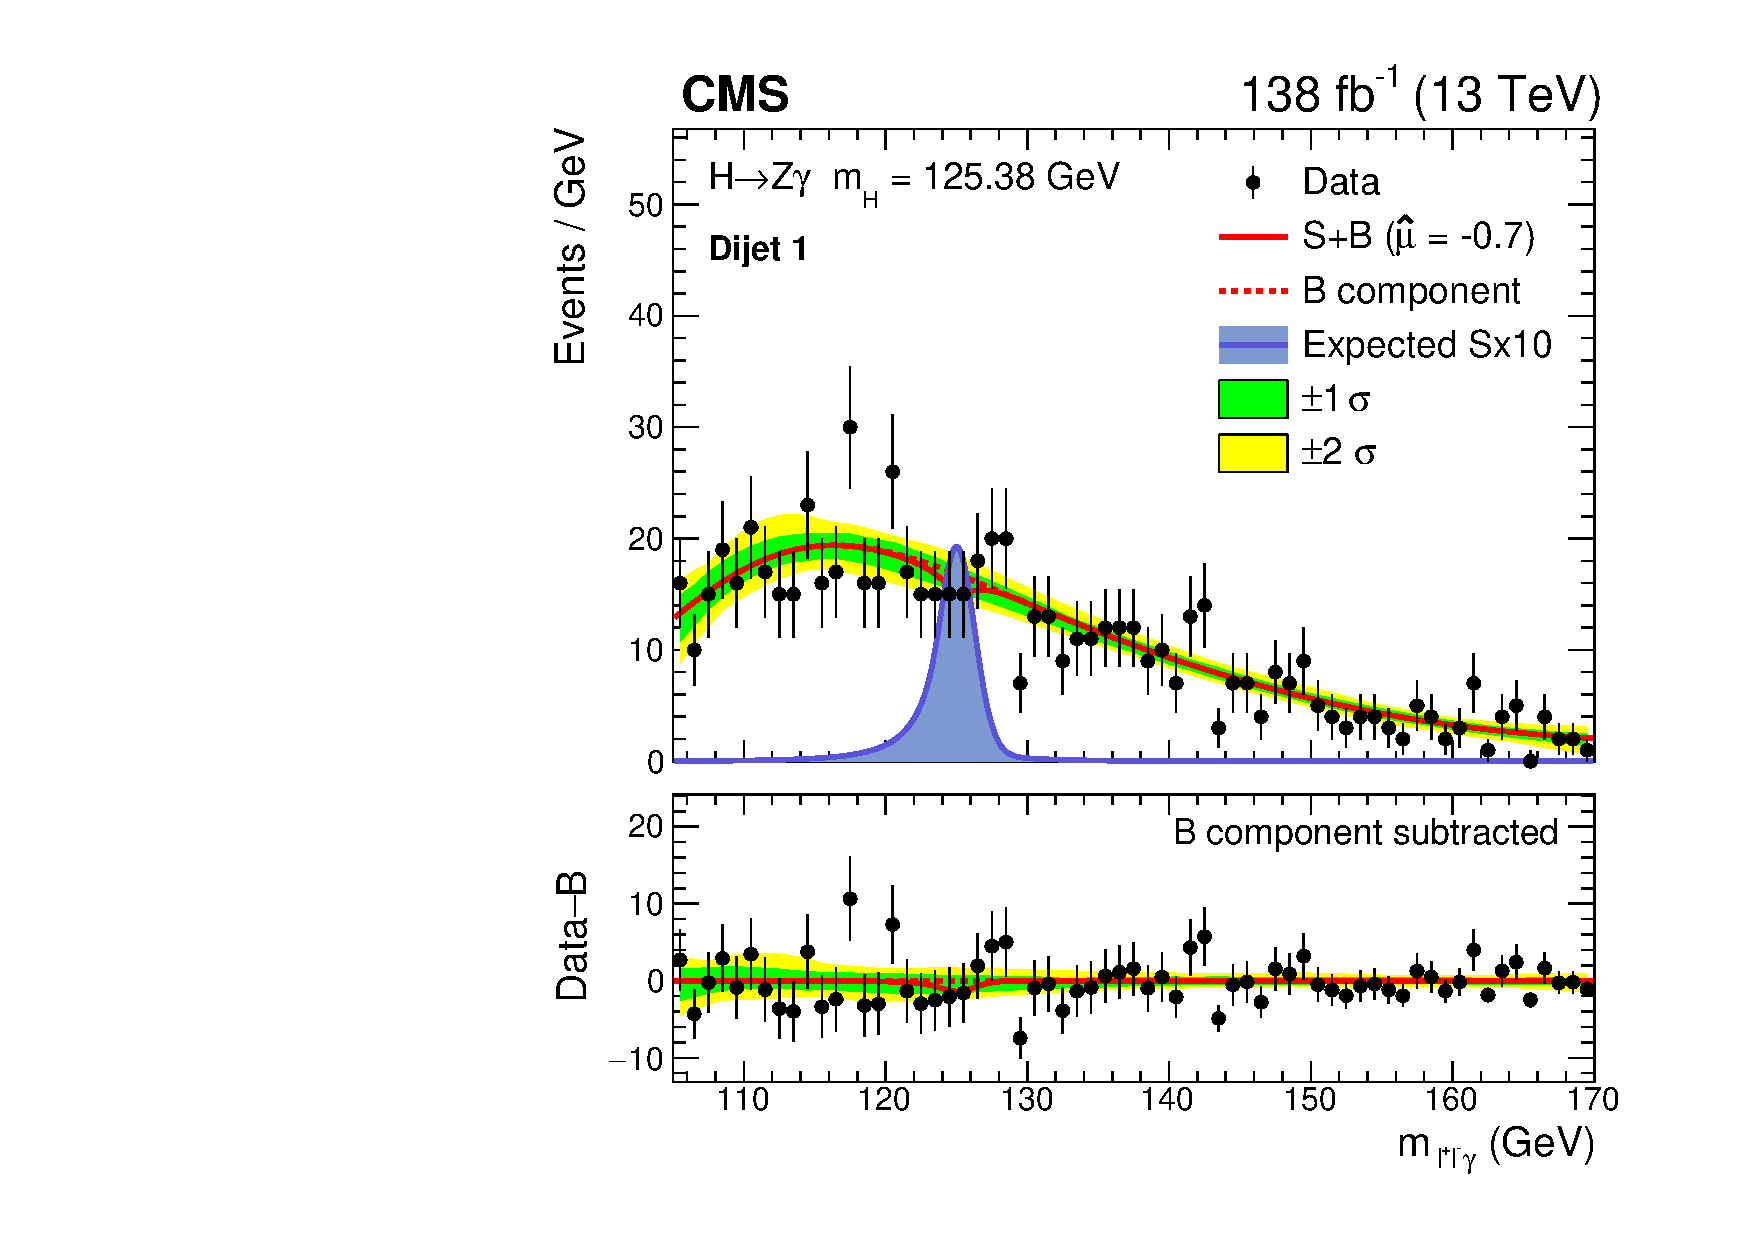
\includegraphics[width=0.45\textwidth]{fig/results/Figure_004-a.pdf}\\
  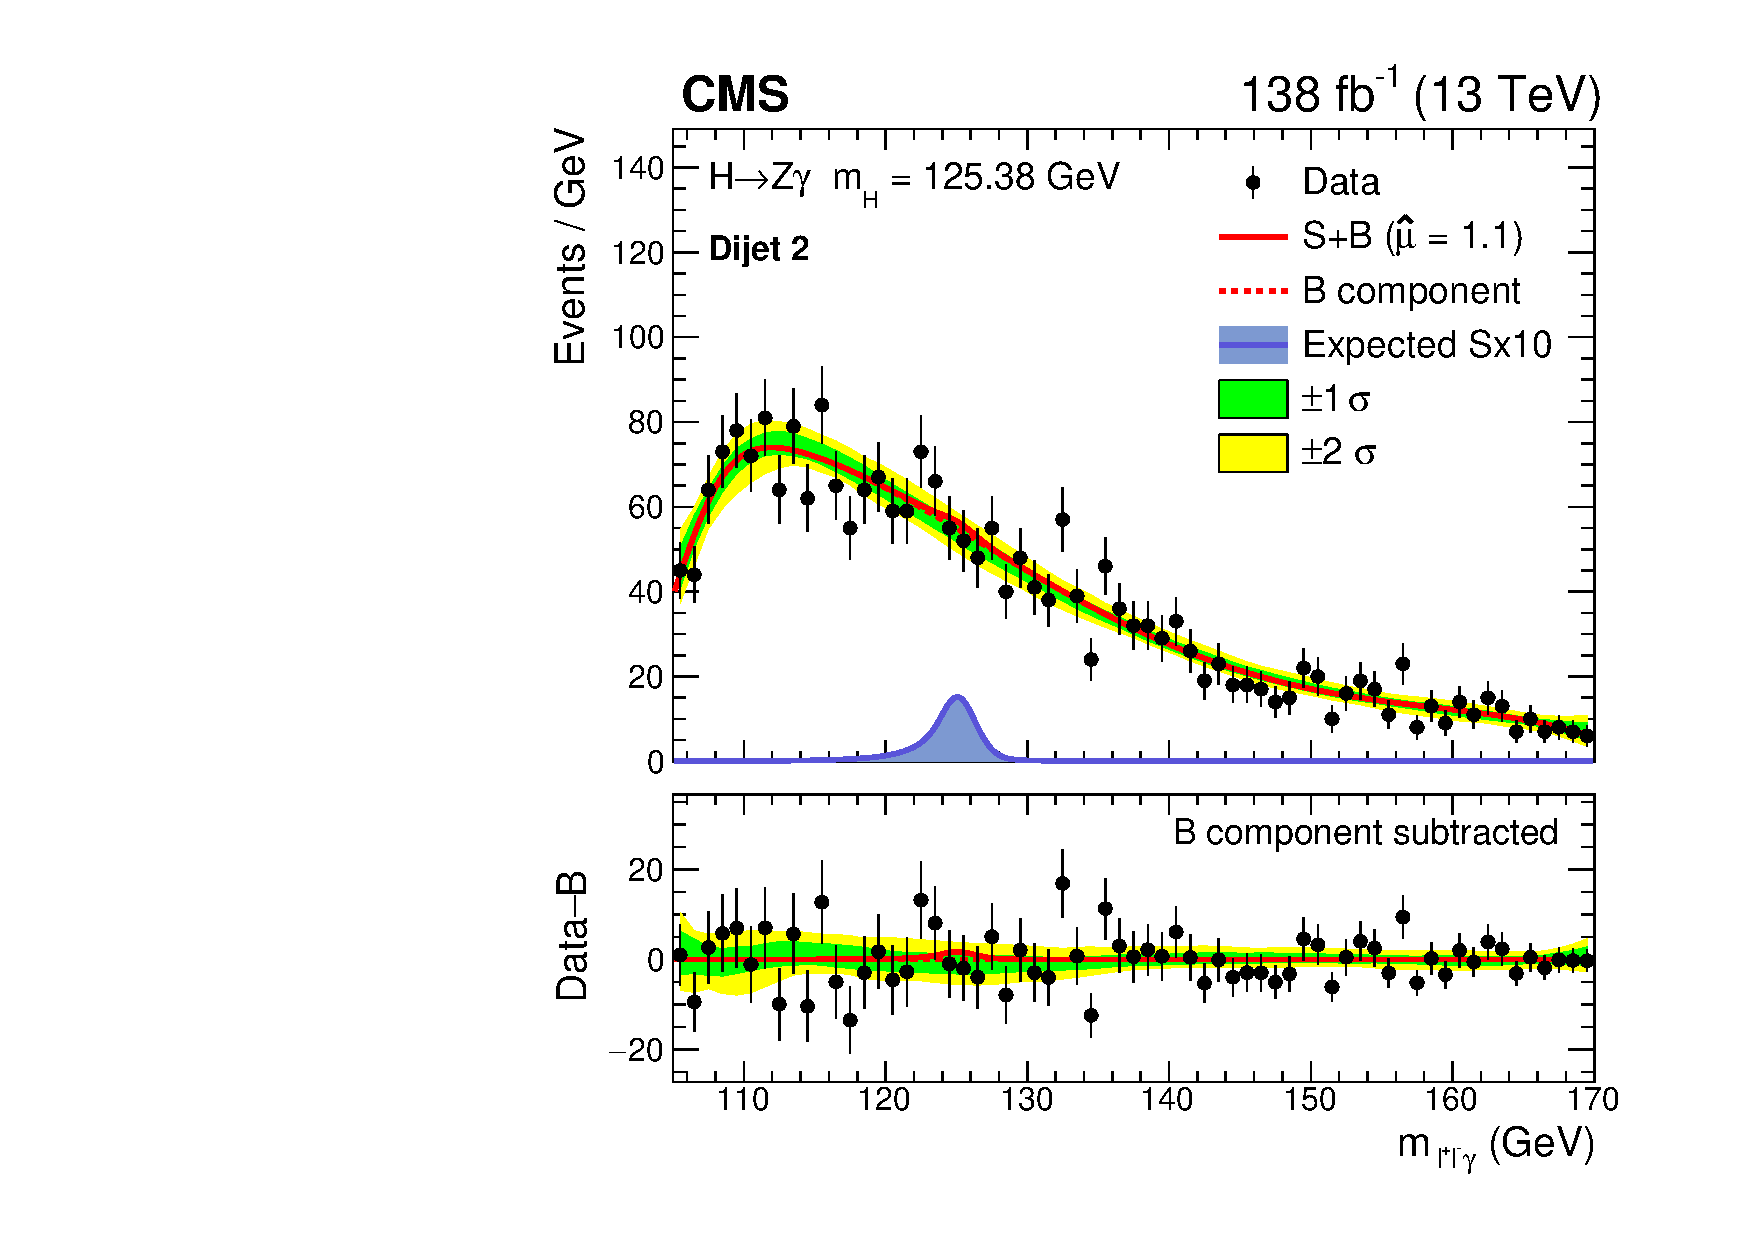
\includegraphics[width=0.45\textwidth]{fig/results/Figure_004-b.pdf}
  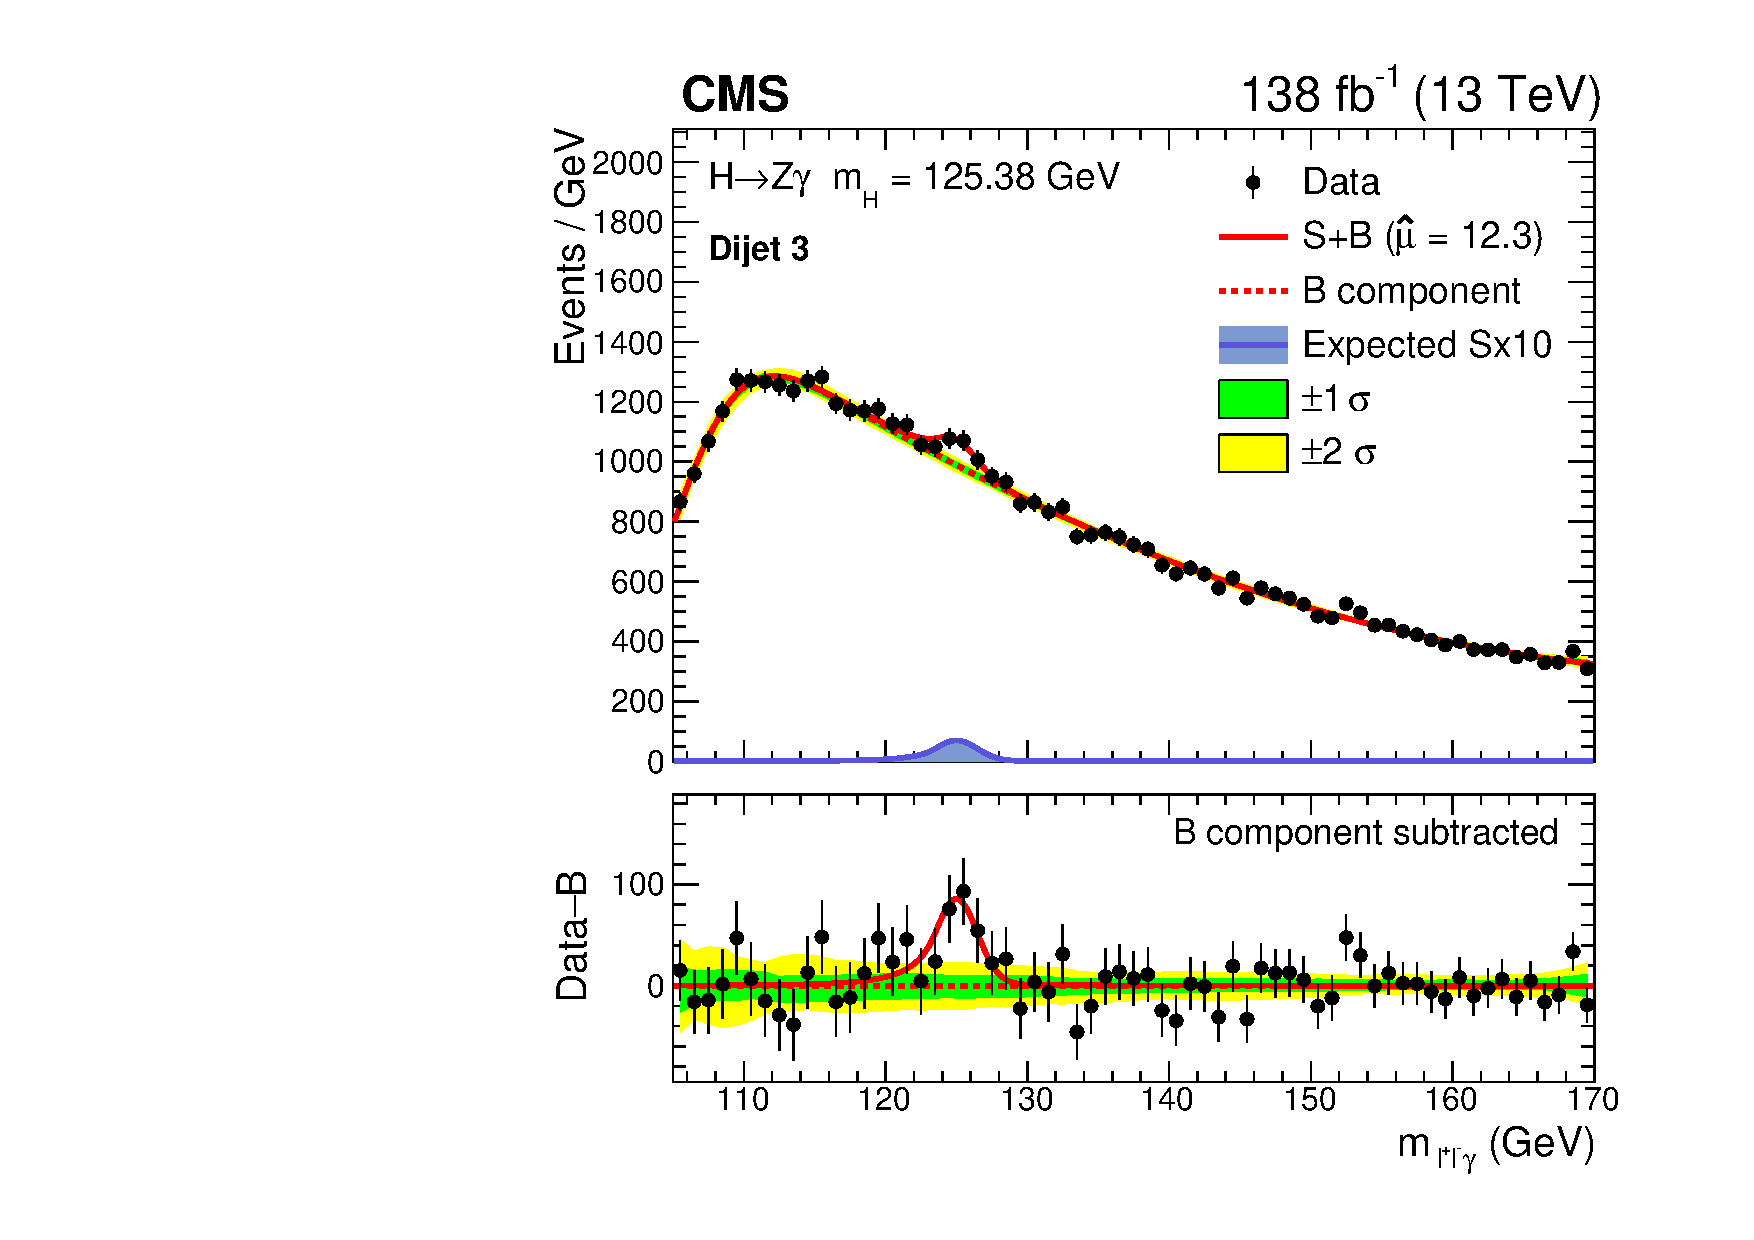
\includegraphics[width=0.45\textwidth]{fig/results/Figure_004-c.pdf}\\
   \caption{Fits to the $m_{\ell^+\ell^-\gamma}$ data distribution
    in the lepton-tagged (upper left), dijet 1 (upper right), dijet 2 (lower left), and
  dijet 3 (lower right) categories.
  In the upper panel, the red solid line shows the result of a signal-plus-background fit to the given category.
  The red dashed line shows the background component of the fit.
  The green and yellow bands represent the $68$ and $95$\% \CL\ uncertainties in the fit.
  Also plotted is the expected SM signal, scaled by a factor of 10.
  In the lower panel, the data minus the background component of the fit is shown. \label{fig:3}}
  \end{figure}

  \begin{figure}
  \centering
  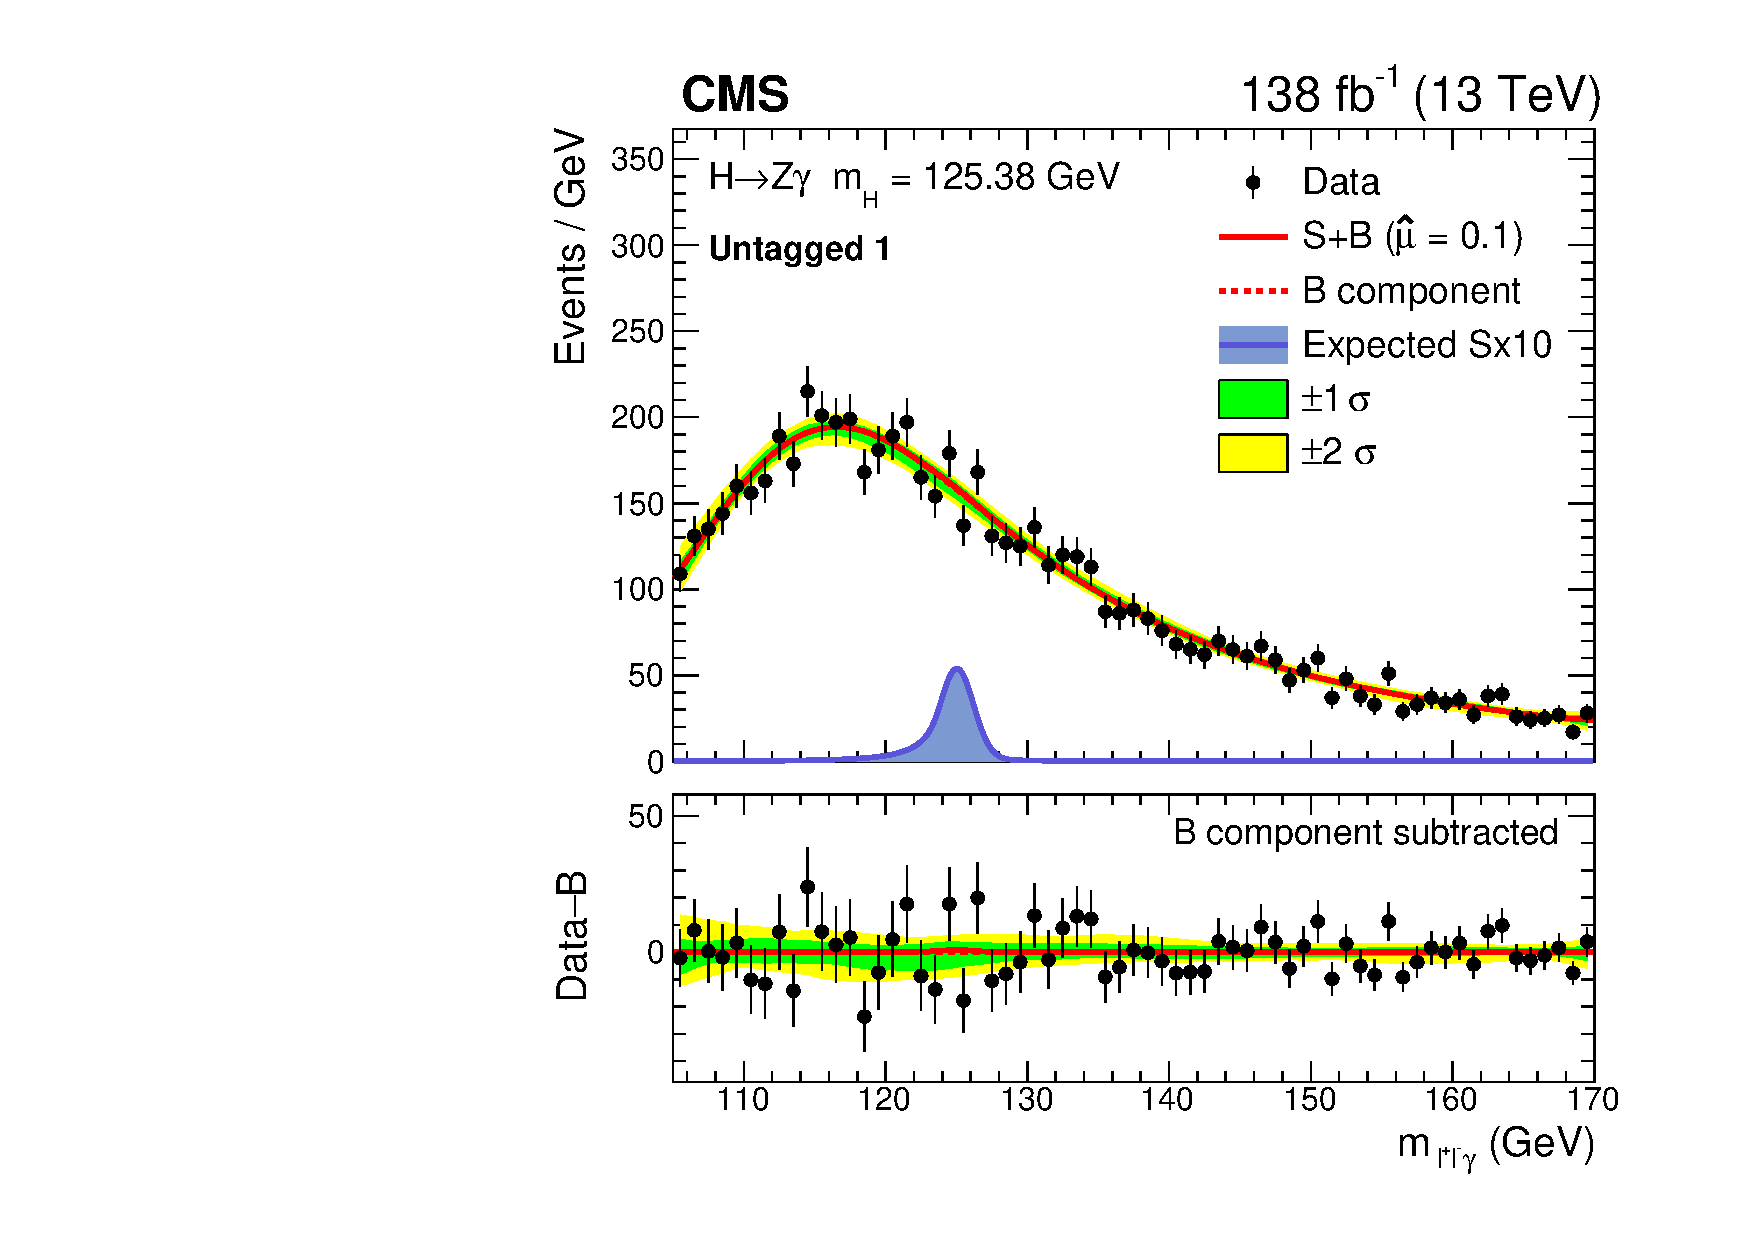
\includegraphics[width=0.45\textwidth]{fig/results/Figure_006-a.pdf}
  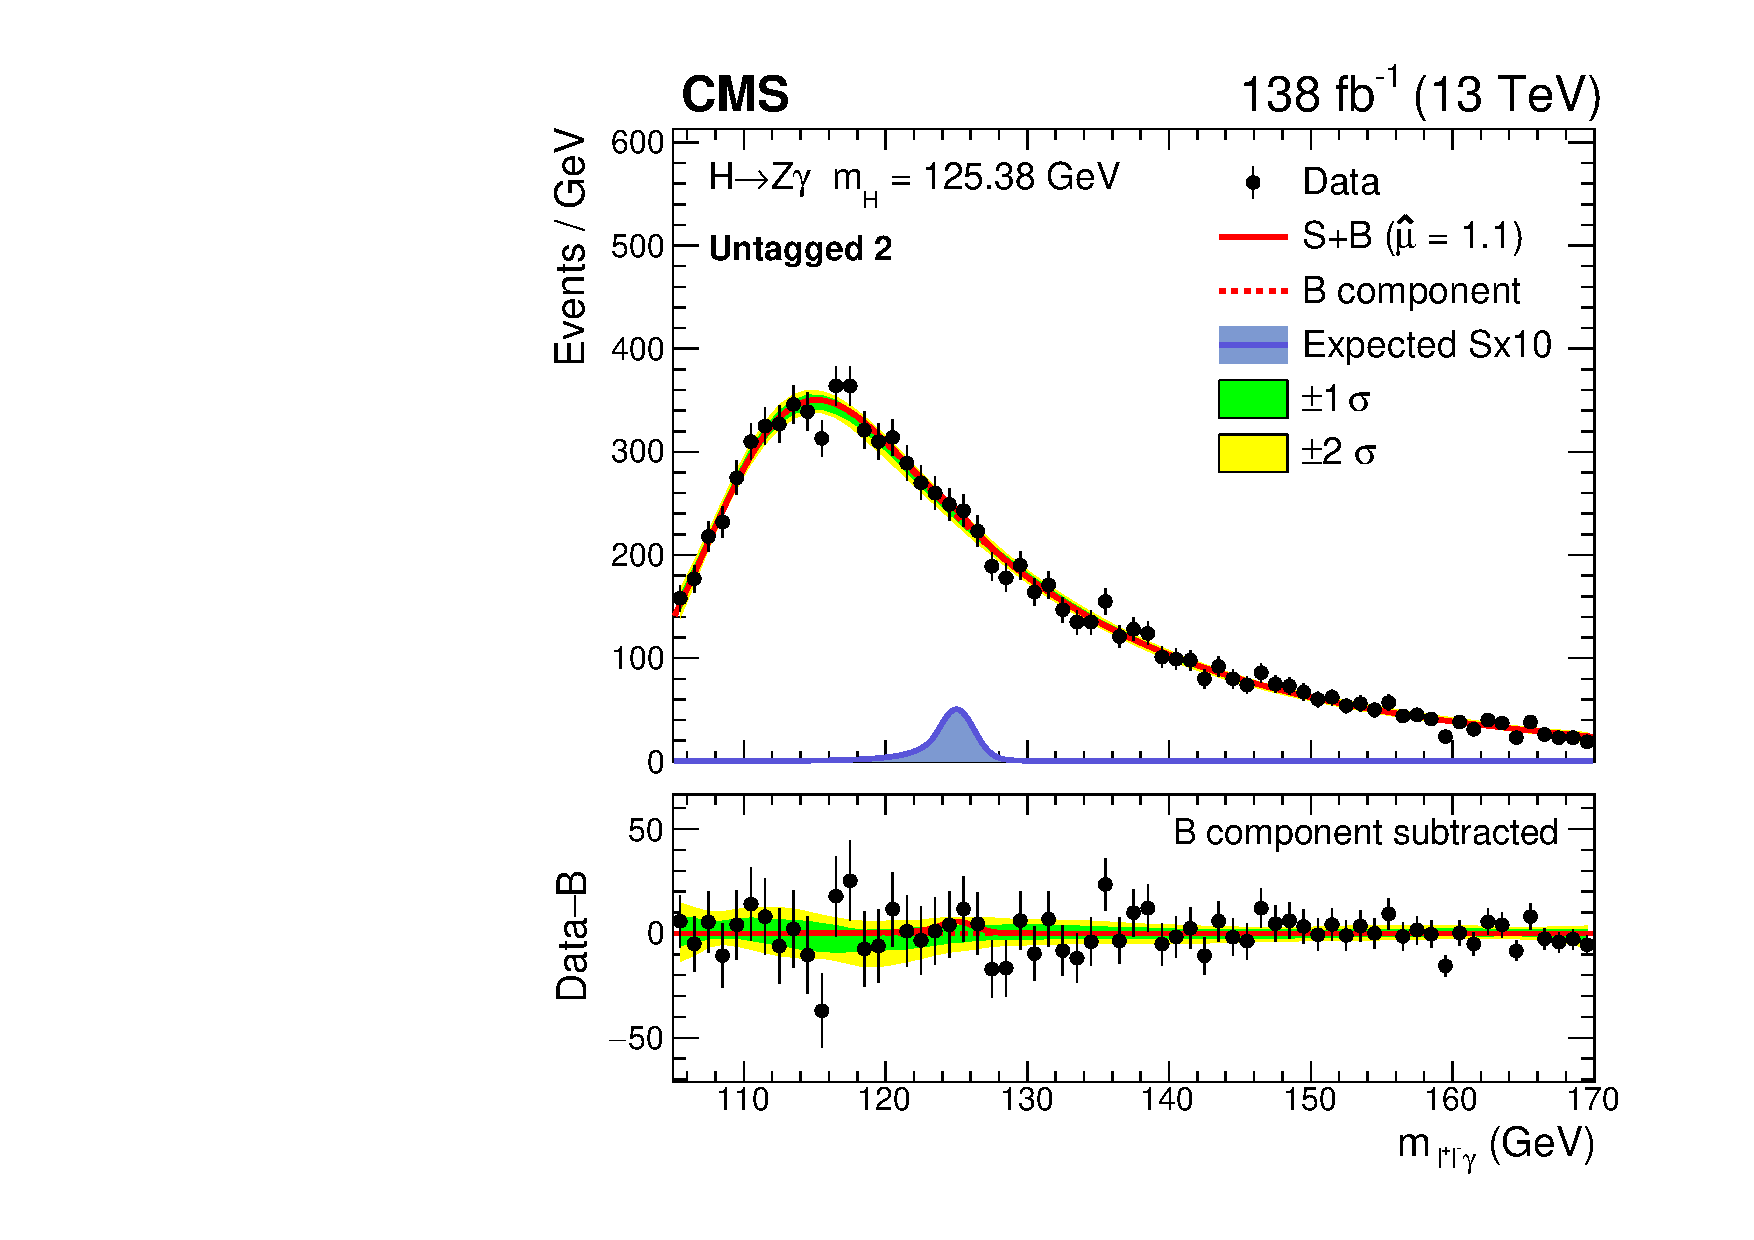
\includegraphics[width=0.45\textwidth]{fig/results/Figure_006-b.pdf}\\
  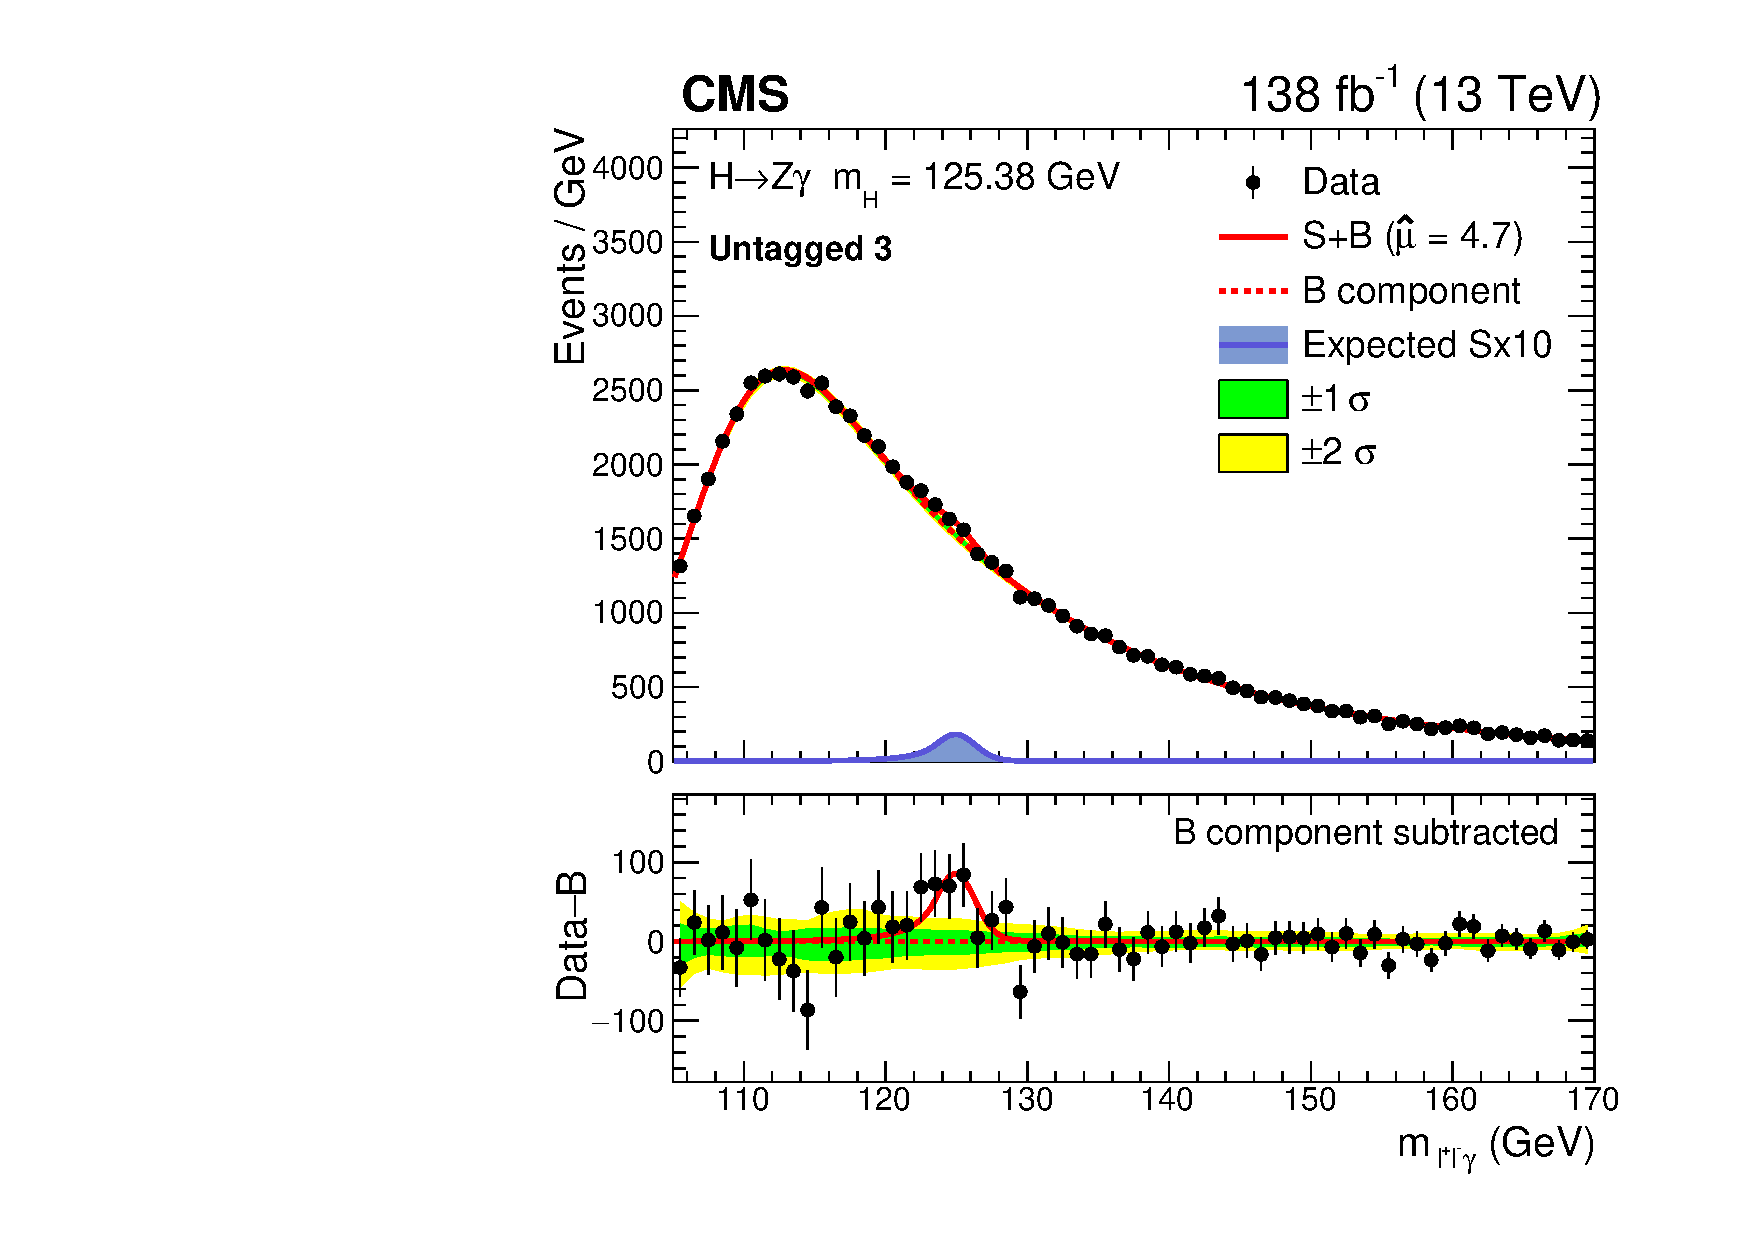
\includegraphics[width=0.45\textwidth]{fig/results/Figure_006-c.pdf}
  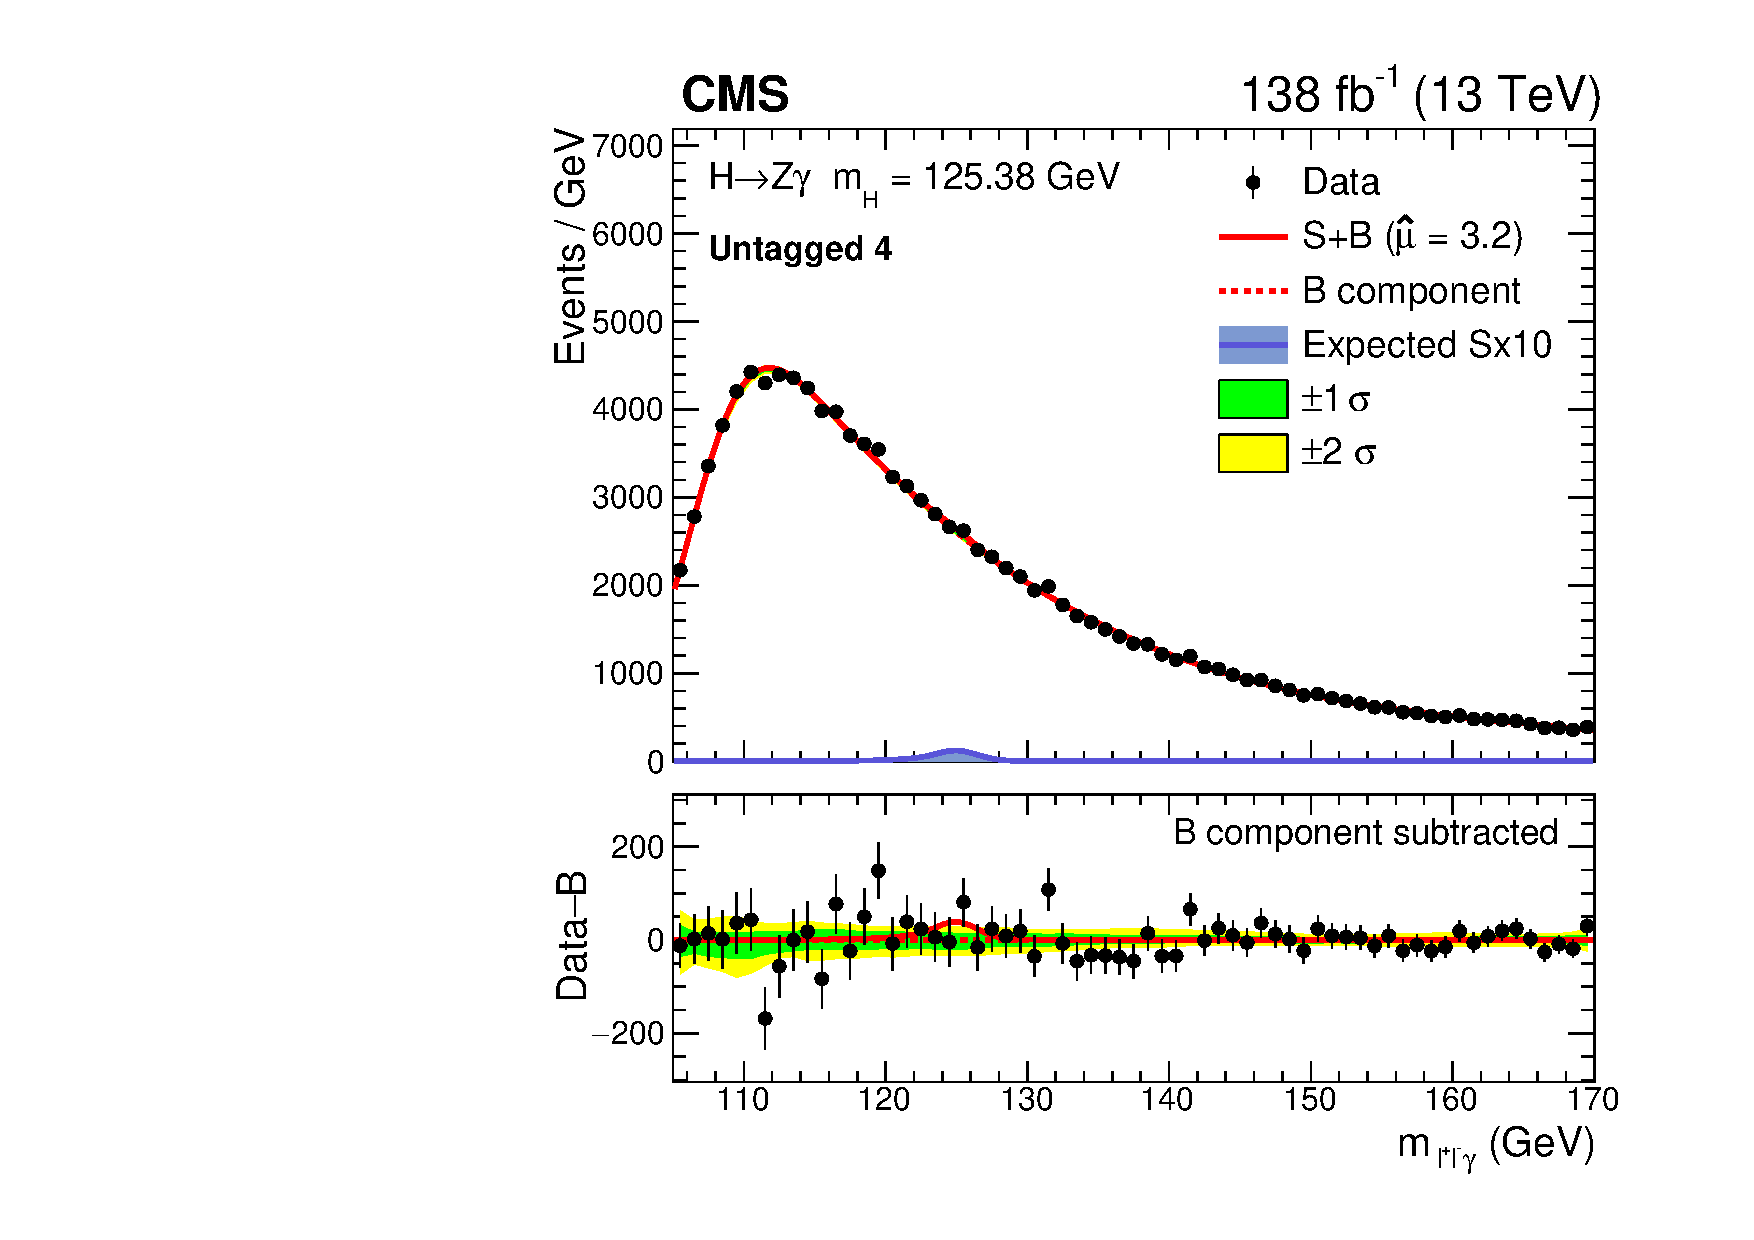
\includegraphics[width=0.45\textwidth]{fig/results/Figure_006-d.pdf}
   \caption{Fits to the $m_{\ell^+\ell^-\gamma}$ data distribution
    in the untagged 1 (upper left), untagged 2 (upper right), untagged 3 (lower left), and
  untagged 4 (lower right) categories.
  In the upper panel, the red solid line shows the result of a signal-plus-background fit to the given category.
  The red dashed line shows the background component of the fit.
  The green and yellow bands represent the $68$ and $95$\% \CL\ uncertainties in the fit.
  Also plotted is the expected SM signal, scaled by a factor of 10.
  In the lower panel, the data minus the background component of the fit is shown. \label{fig:4}}
  \end{figure}

\begin{figure}
\centering
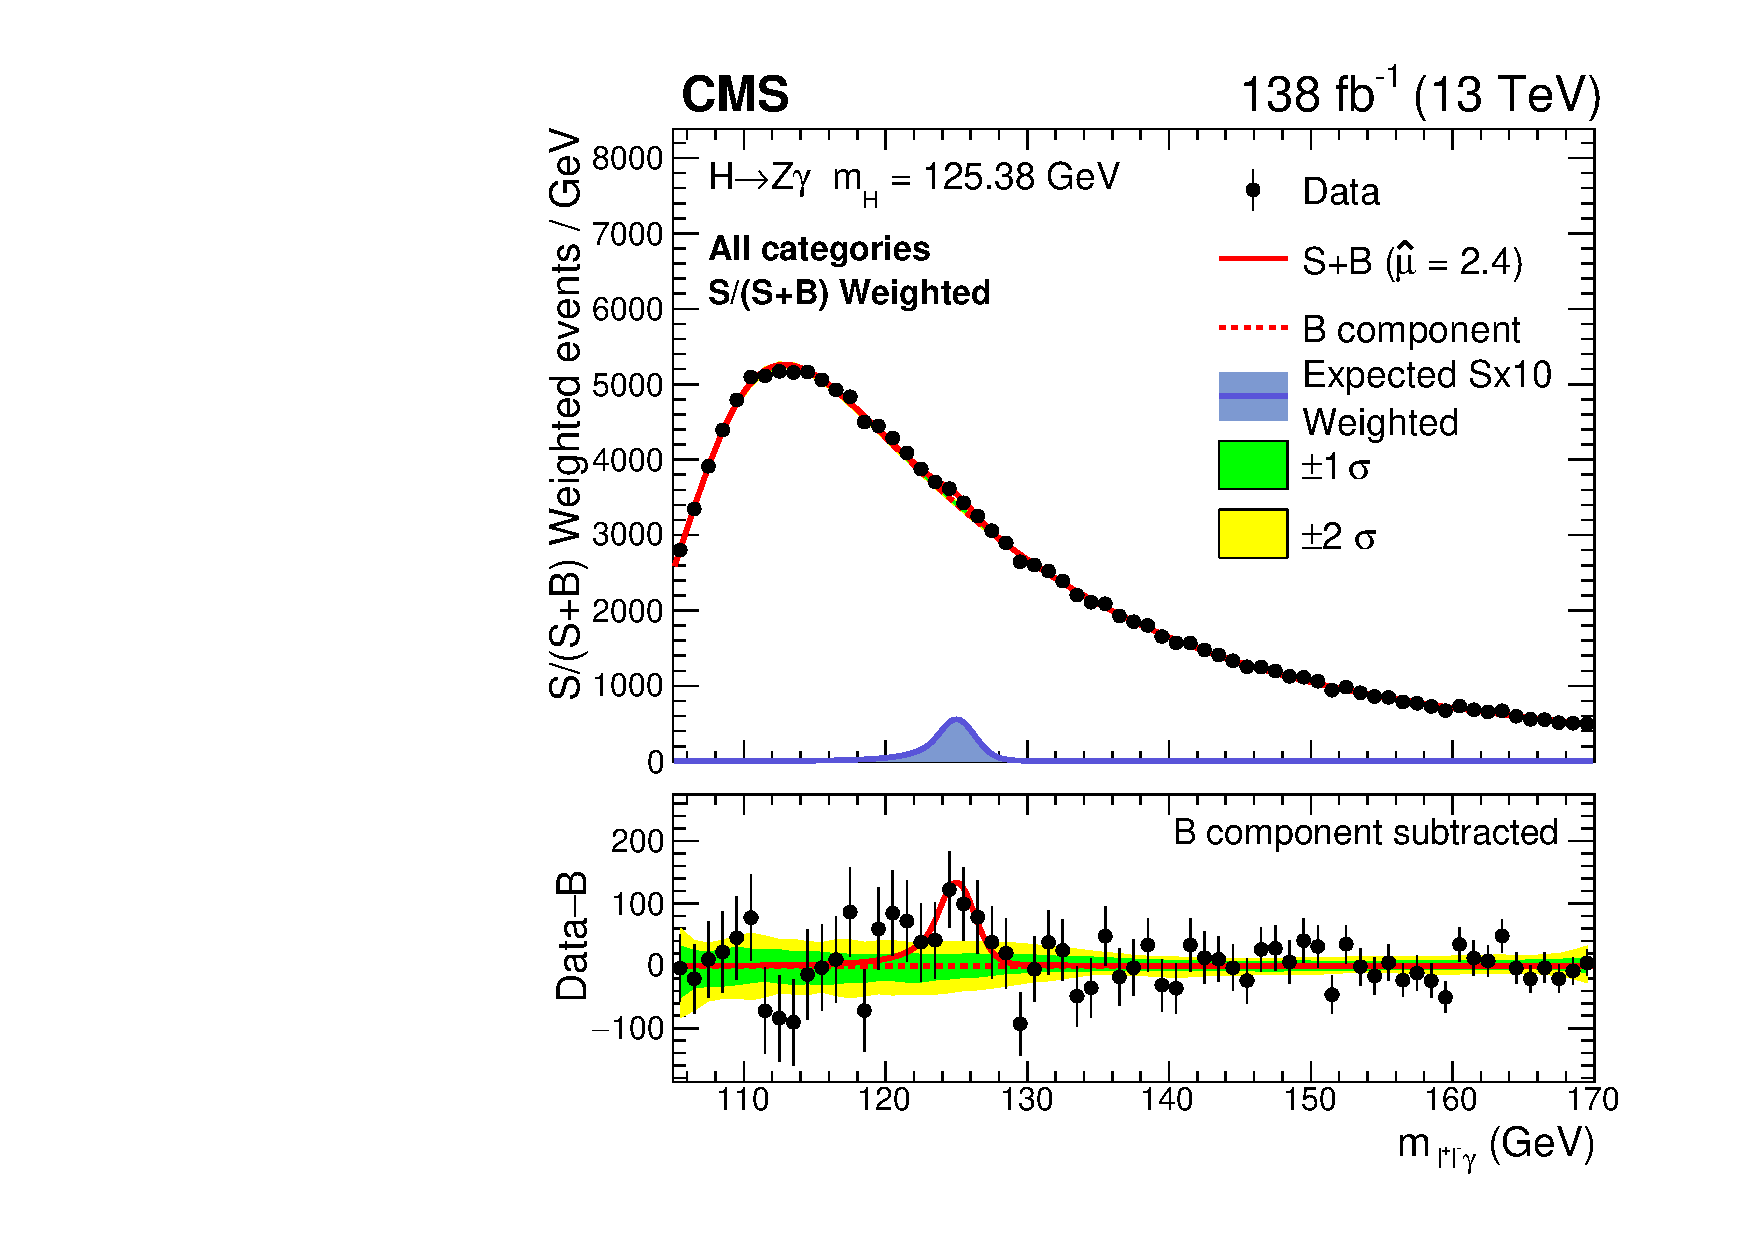
\includegraphics[width=0.5\textwidth]{fig/results/Figure_012.pdf}
 \caption{Sum over all categories of the data points and signal-plus-background model after the simultaneous fit to each $m_{\ell^+\ell^-\gamma}$ distribution. 
 The contribution from each category is weighted by $S/(S+B)$, as defined in the text. 
 In the upper panel, the red solid line shows the signal-plus-background fit. The red dashed line shows the background component of the fit. The green and yellow bands represent the $68$ and $95$\% CL uncertainties in the fit. Also plotted is the expected SM signal weighted by $S/(S+B)$ and scaled by a factor of 10. In the lower panel, the data minus the background component of the fit is shown.
   }
\label{fig:SignalBackground}
\end{figure}

The best fit value of the signal strength is $\signalstrengthExpanded$ at $m_\PH=\mH$\GeV.
The corresponding measured value of $\sigma(\Pp\Pp\to\PH)\mathcal{B}(\PH\to\PZ\gamma)$ is $\brExpanded$\,pb. This measurement is consistent with the SM prediction of $0.09 \pm 0.01$\,pb at the \compatibility\, standard deviation level.
Figure~\ref{fig:lim-combo125} shows the signal strengths obtained for each category separately, corresponding to the fit results shown in Figs.~\ref{fig:3} and \ref{fig:4}, as well as from simultaneous fits to the dijet categories, the untagged categories, and all categories combined. 
Among the eight categories, dijet 1 is the most sensitive.
A category compatibility $\textit{p}$-value, under the hypothesis of a common signal strength in all categories, is calculated from the likelihood ratio between the 
nominal combined fit, in which all categories have the same signal strength parameter, 
and a separate fit, in which each category has its own signal strength parameter. 
This $\textit{p}$-value is found to be \channelcompatp, corresponding to \channelcompatsigma\, standard deviations, and is driven by the dijet 3 category, which has a signal strength of $\hat{\mu}=\signalstrengthdijetthree$. 
The observed (expected) local significance is \obssig\,(\expsig) standard deviations. 
Upper limits on $\mu$ are calculated at 1\GeV intervals 
in the mass range of $120 < m_{\ell^+\ell^-\gamma} < 130\GeV$ and at $m_\PH=\mH\GeV$, as shown in Fig.~\ref{fig:lim}.
The observed (expected) limit at 95\% CL relative to the SM expectation for $m_\PH=\mH\GeV$ is $\obslimit$ ($\explimit$). 

\begin{figure}
  \centering
  %  \includegraphics[width=0.75\textwidth]{Figure_010.pdf}
   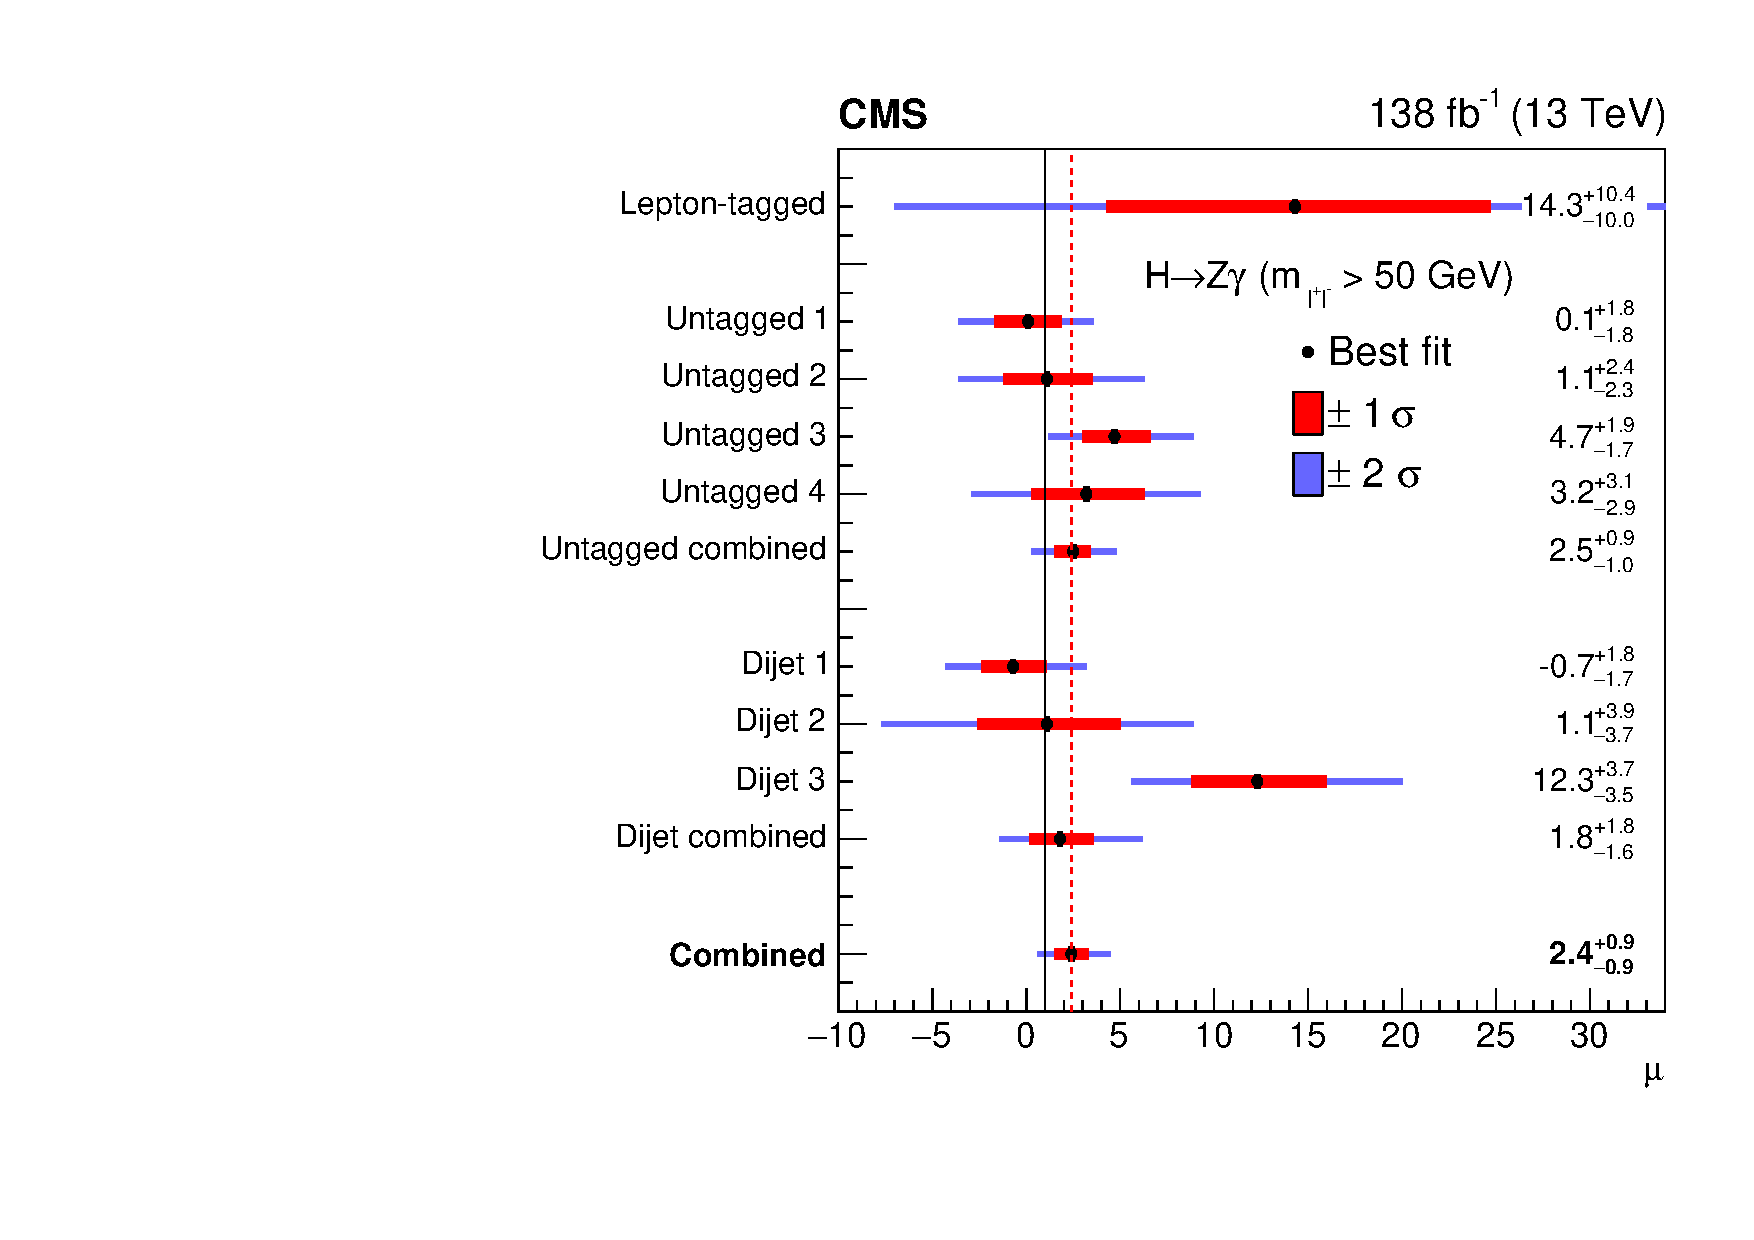
\includegraphics[width=0.7\textwidth]{fig/results/Figure_011.pdf}
    \caption{
Observed signal strength ($\mu$) for a SM Higgs boson with $m_\PH=\mH\GeV$. 
The labels ``untagged combined," ``dijet combined," and ``combined" represent the results obtained from simultaneous fits of the untagged categories, dijet categories, and full set of categories, respectively. 
%Fits perform simultaneously for the combined categories, where the untagged, dijet and all categories are considered. 
The black solid line shows $\mu=1$, and the red dashed line shows the best fit value $\hat{\mu}=\,$\signalstrength ~of all categories combined.
    \label{fig:lim-combo125}}
\end{figure}

\begin{figure}
  \centering
  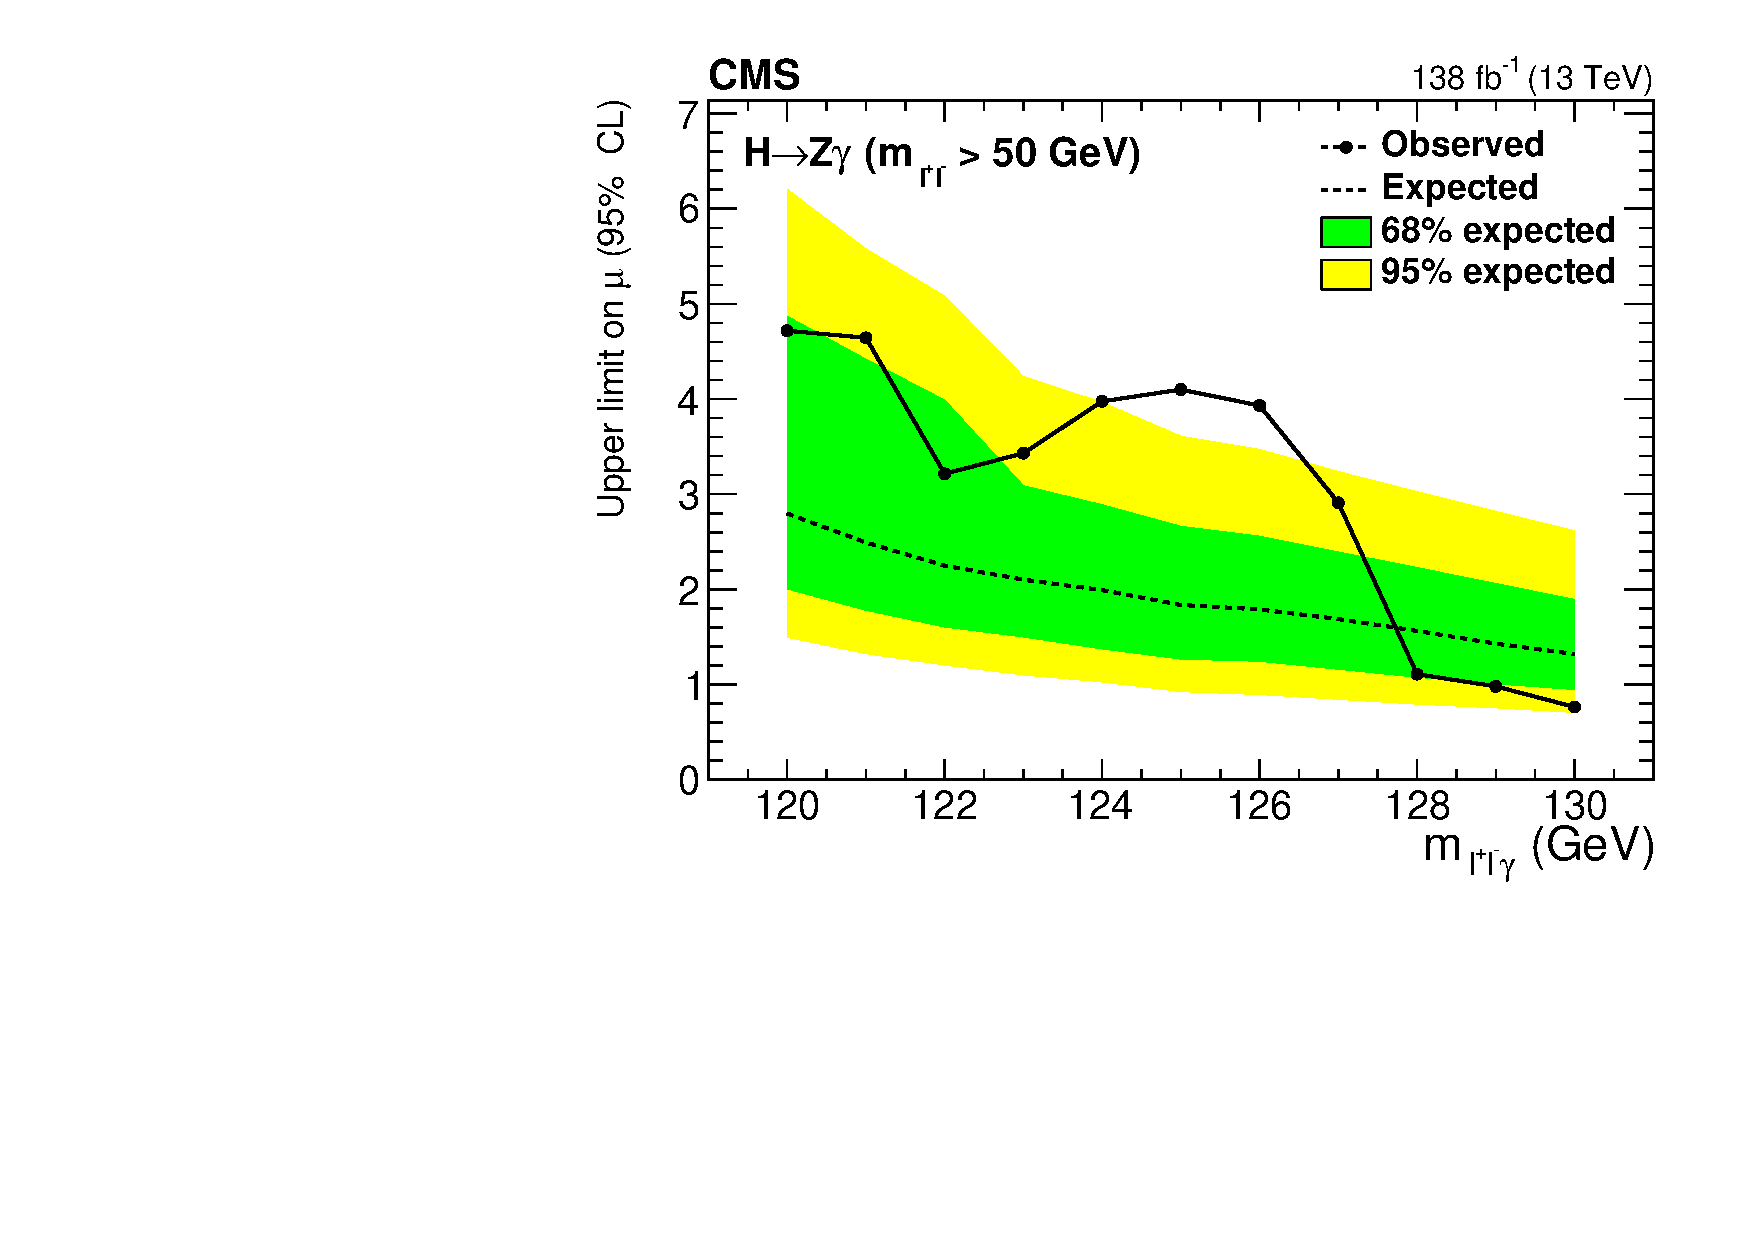
\includegraphics[width=0.7\textwidth]{fig/results/Figure_009.pdf}
    \caption{
	    Upper limit ($95$\%~\CL) on the signal strength ($\mu$) relative to the SM prediction, as a function of the assumed value of the Higgs boson mass used in the fit.
    \label{fig:lim}}
\end{figure}

\section{Ratio Measurement}
The ratio $\mathcal{B}(H\rightarrow\PZ\gamma)/\mathcal{B}(H\rightarrow\gamma\gamma)$ is theoretically interesting, as it is 
potentially sensitive to beyond BSM physics, such as supersymmetry and extended Higgs 
sectors~\cite{Djouadi:1996yq,Zg_theory_extension,Zg_theory_decaywidth}.
BSM effects from models such as these typically shift the $H\rightarrow\PZ\gamma$ and $\PH\to\PGg\PGg$ branching fractions 
by different amounts, making the ratio the most sensitive observable. 
By combining the $H\rightarrow\PZ\gamma$ analysis with the existing CMS $\PH\to\PGg\PGg$ analysis, described in Ref.~\cite{CMS:2021kom}, 
we can obtain a measurement of this ratio and compare it to the SM prediction of $0.69 \pm 0.04$. An experimental advantage 
of this measurement is the cancellation of common theoretical uncertainties related to Higgs boson production and common experimental 
uncertainty sources like the L1 prefiring issue.

The ratio measurement is obtained via a combined fit of the two analyses with two parameters of interest: the $\PH\to\PGg\PGg$ signal 
strength with respect to the SM expectation ($\mu_{\gamma\gamma}$) and the ratio of the signal strengths for the two channels
($\mu_{Z\gamma} / \mu_{\gamma\gamma}$). After obtaining the best fit values for these parameters of interest, 
the ratio of signal strengths can be scaled to obtain the ratio of branching fractions. Common systematic uncertainties in the two 
analyses are correlated in the combined fit, and are listed in Table \ref{tab:corr_unc}. The combination is performed at 
a Higgs boson mass of 125.38 GeV, and discrete profiling of the background models is enabled for both analyses. 

The profile likelihood scans for the parameters of interest are shown in Figure \ref{fig:scan_br}. The best fit values of the 
parameters of interest are $\mu_{\gamma\gamma} = 1.121^{+0.095}_{-0.090}$ and 
$\mu_{Z\gamma}/\mu_{\gamma\gamma} = 2.225^{+0.926}_{-0.825}$. 
The value of $\mu_{\gamma\gamma}$ agrees well with the standalone $\PH\to\PGg\PGg$ fit. 
Multiplying through, the value of $\mu_{Z\gamma}$ is 2.49, which 
agrees well with the result of the standalone $H\rightarrow\PZ\gamma$ fit.
The measured value of $\mathcal{B}(\PH\to\PZ\gamma)/\mathcal{B}(\PH\to\gamma\gamma)$ from the combined fit with the $\PH\to\PGg\PGg$
analysis is \brRatio. This measurement is consistent with the SM prediction for the ratio at the \brRatioCompat\, standard deviation level. 
The nuisance parameter impacts on the signal strength ratio are shown in Figure \ref{fig:ratio_impacts}.

\begin{table}
   \centering   
   % \resizebox{\textwidth}{15mm}{
      
\begin{tabular}{cc}
   Source &\\\hline
   Theoretical uncertainties&\\\\
   Scale uncertainties  &  QCD scale ZH\\
                        &  QCD scale WH\\
                        &  QCD scale ggH\\
                        &  QCD scale qqH\\
                        &  QCD scale ttH\\
   PDF uncertainties    &  pdf\_Higgs\_ggH\\
                        &  pdf\_Higgs\_VH\\
                        &  pdf\_Higgs\_qqH\\
                        &  pdf\_Higgs\_ttH\\\hline
   Systematic uncertainties&\\\\
   Luminosity  &lumi\_13TeV\_Uncorrelated\_2016,2017,2018\\
                            &lumi\_13TeV\_Beam\_Current\_Calibration\\
                            &lumi\_13TeV\_Beam\_Beam\_Deflection\\
                            &lumi\_13TeV\_Dynamic\_Beta\\
                            &lumi\_13TeV\_Ghosts\_And\_Satellite\\
                            &lumi\_13TeV\_Length\_Scale\\
                            &lumi\_13TeV\_X\_Y\_Factorization\\
   Parton showering        &PartonShower\_norm\\
   Underlying events        &UnderlyingEvent\_norm\\
   L1-prefire           &2016,2017 L1 prefire uncertainty\\
                        

\end{tabular}
% }
\caption{Correlated uncertainties between $\PH\to\cPZ\gamma$ and $\PH\to\gamma\gamma$ for the $\mathcal{B}(\PH\to\cPZ\gamma)/\mathcal{B}(\PH\to\gamma\gamma)$ measurement.}
\label{tab:corr_unc}
\end{table}

\begin{figure}
   \begin{center}
   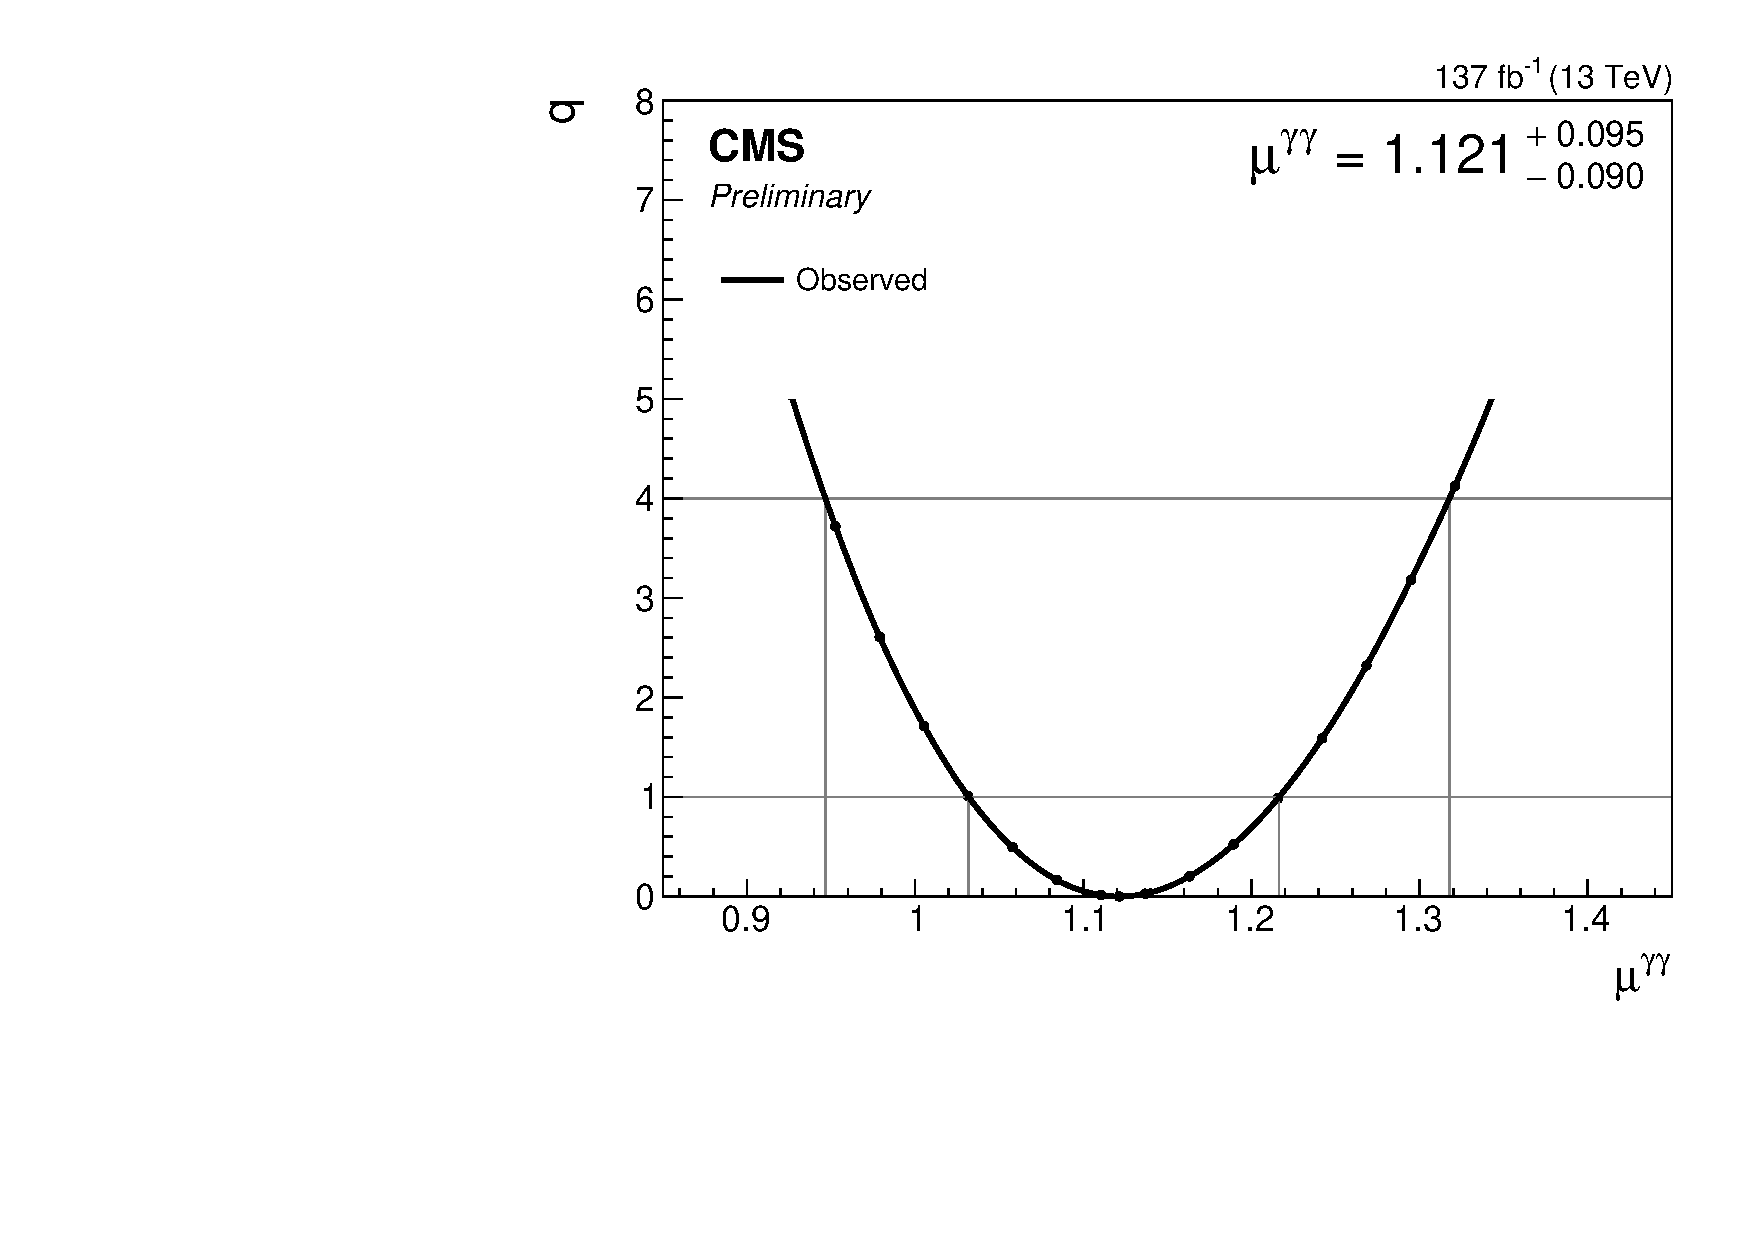
\includegraphics[width=0.45\textwidth]{fig/results/ratio/scan_mu_BR_gamgam.pdf}
   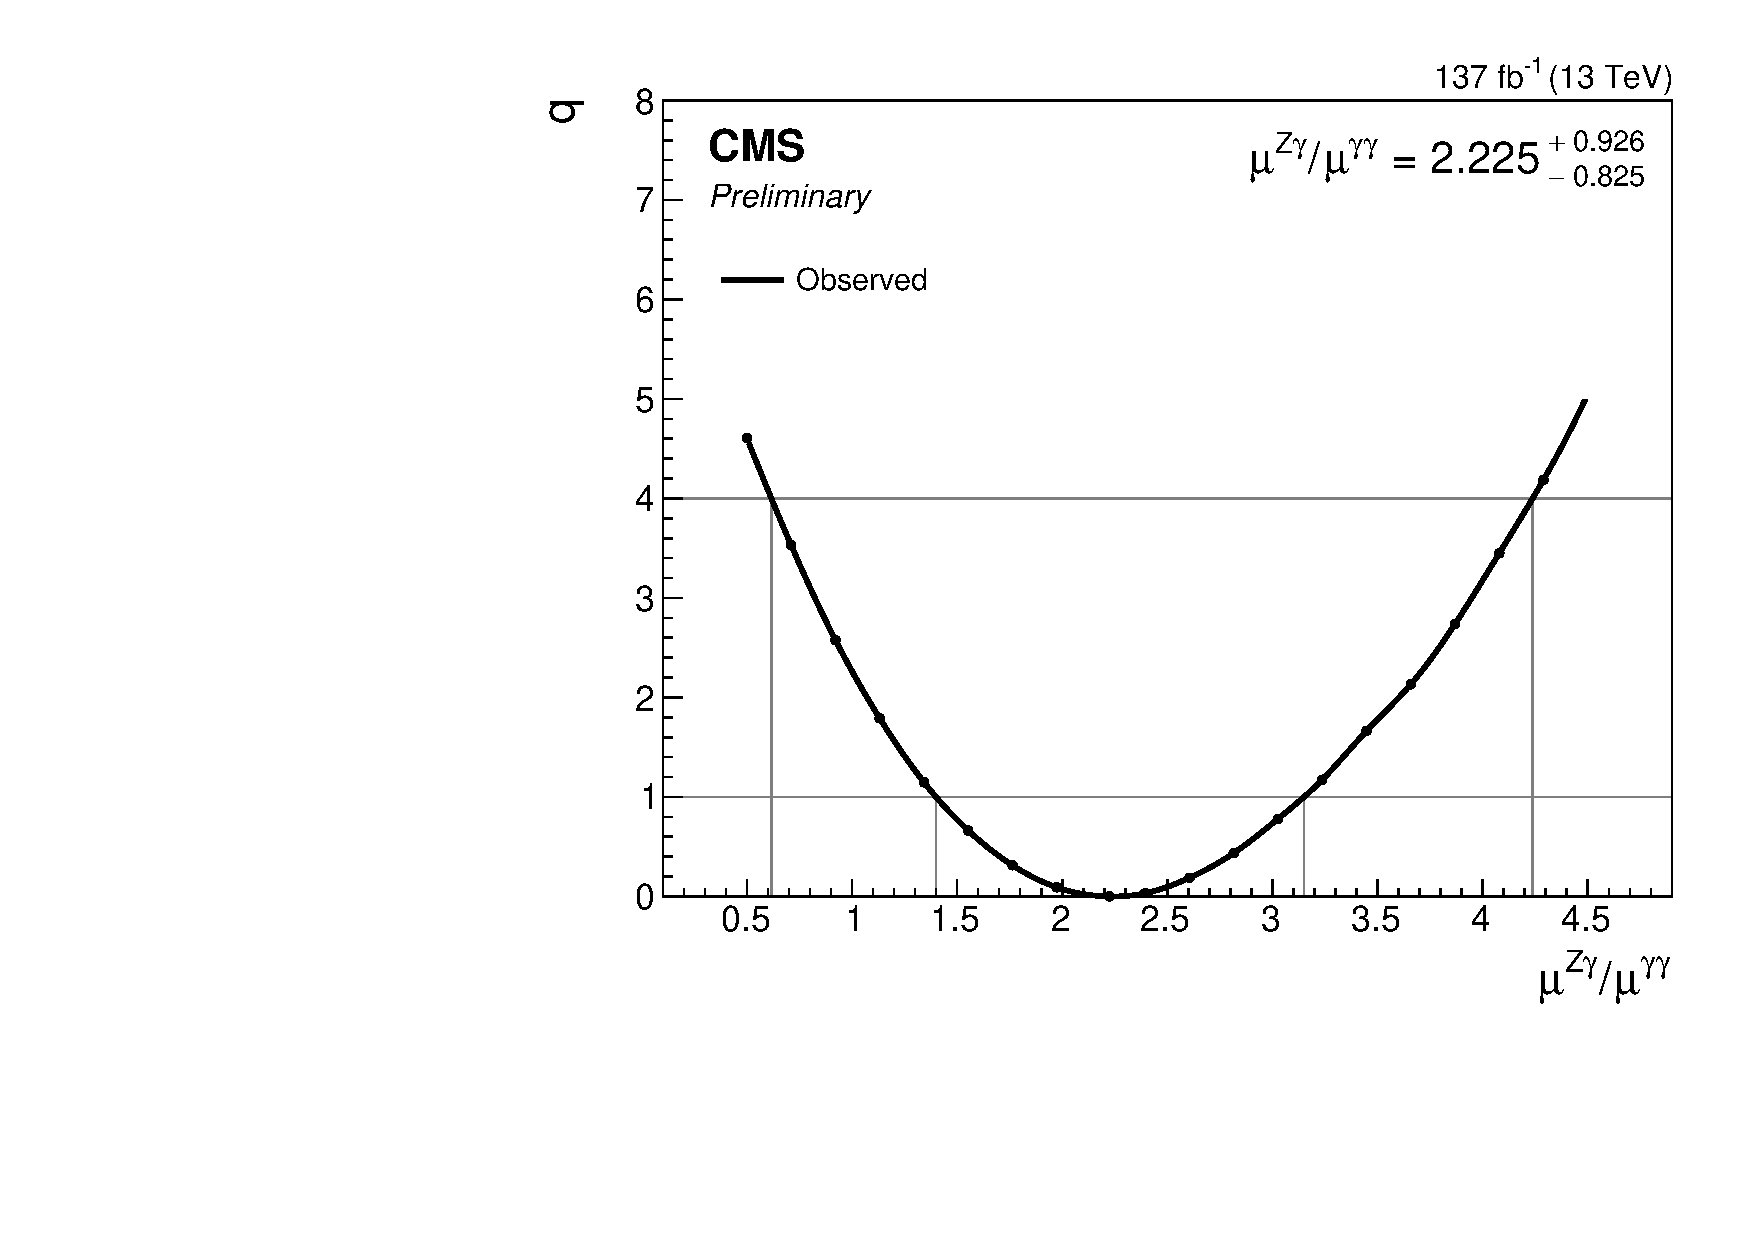
\includegraphics[width=0.45\textwidth]{fig/results/ratio/scan_mu_BR_Zgam_r_BR_gamgam.pdf}\\
   \caption{Profile likelihood scans of $\mu_{\gamma\gamma}$ and $\mu_{\PZ\gamma}/\mu_{\gamma\gamma}$ with fixed $m_H=125.38\GeV$.}
   \label{fig:scan_br}
   \end{center}    
\end{figure}

\begin{figure}
	\ContinuedFloat
   \begin{center}
   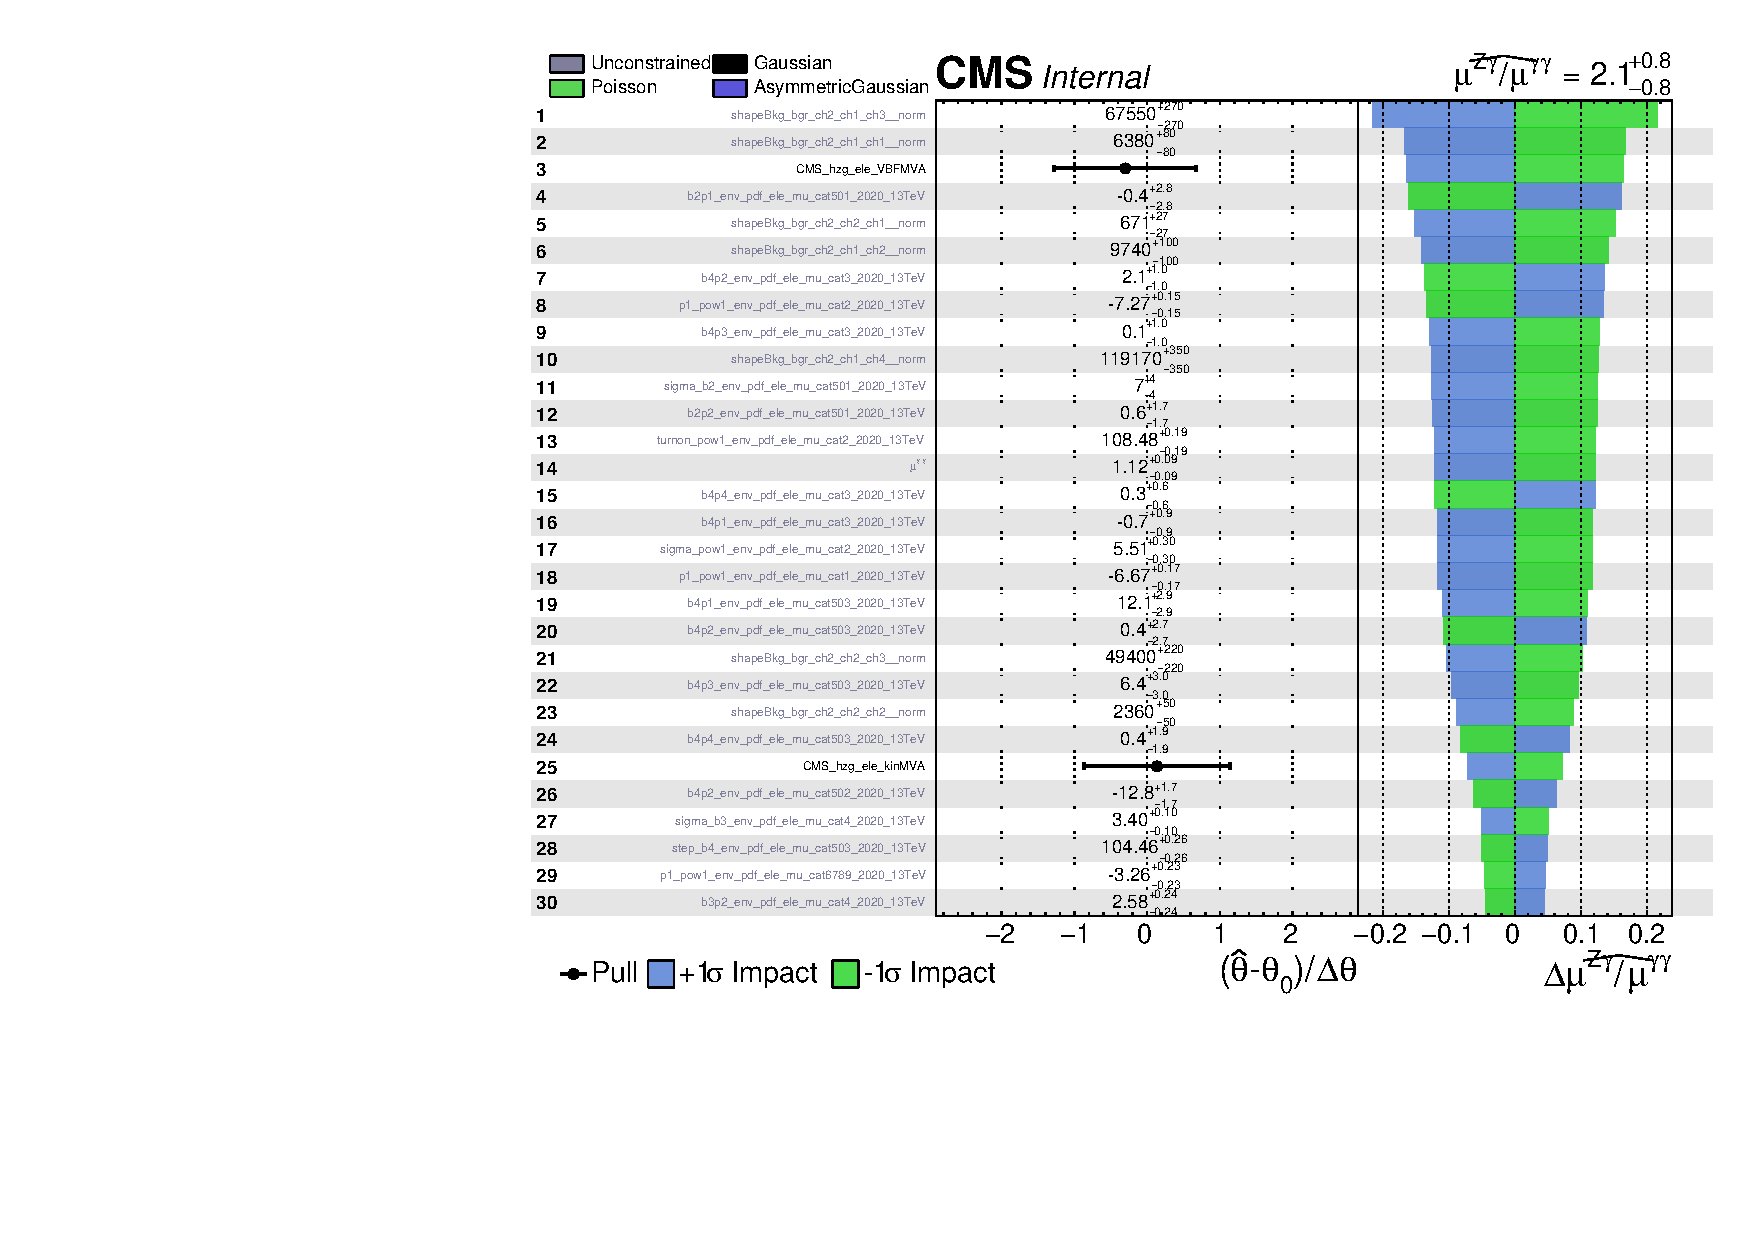
\includegraphics[width=0.75\textwidth,height=0.45\textheight]{fig/results/ratio/impacts_hgghzg_mu_BR_Zgam_r_BR_gamgam_obs_1.pdf}\\
   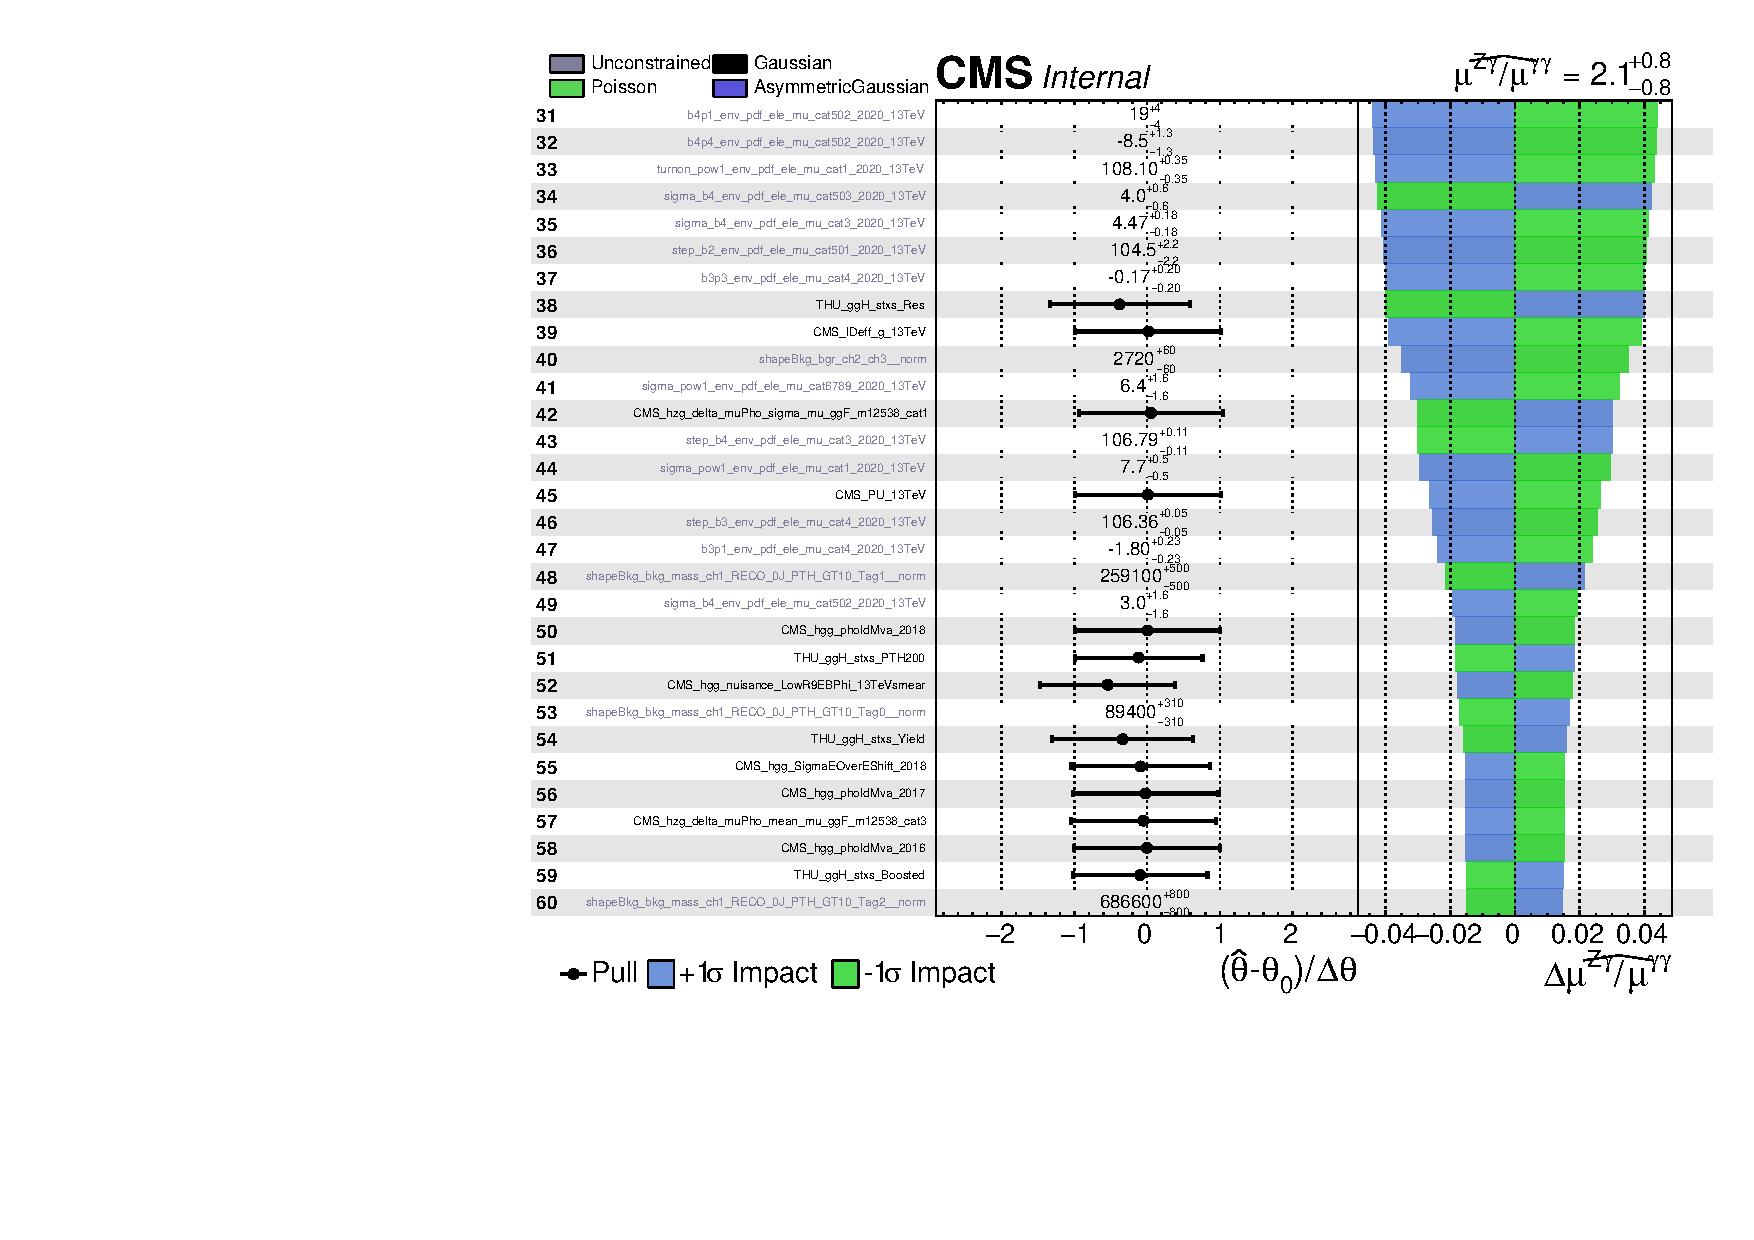
\includegraphics[width=0.75\textwidth,height=0.45\textheight]{fig/results/ratio/impacts_hgghzg_mu_BR_Zgam_r_BR_gamgam_obs_2.pdf}
   \caption{Nuisance parameter impacts on $\mu_{\PZ\gamma}/\mu_{\gamma\gamma}$.}
   \label{fig:ratio_impacts}
   \end{center}    
\end{figure}



% Uncomment the 'singlespace' environment and '\bibsep' command
% if needed - some bibliographic styles overide the definition
% of 'thebibliography' in nuthesis.cls
%
\begin{singlespace}
%\bibsep 12pt
\clearpage\phantomsection % needed for hyperlinks to work correctly
\begin{thebibliography}{xxx}

\bibitem{label1} A bibliographic item.  A bibliographic item.  A
bibliographic item.  A bibliographic item.
\bibitem{label2} Another bibliographic item.  
\bibitem{label3} Yet another bibliographic item.  
% The usages of \bibitem and \cite{..} are 
% explained in Section 4.3 (page 73) of % LaTeX manual.
% Or you may use BibTeX.
\end{thebibliography}
\end{singlespace}

% (The following suggested by Francisco Iacobelli - 5/11/2010)
% In case, you want to use BibTeX, you should replace (or comment)
% the bibliography environment.
% Instead uncomment the following lines and replace <bib file>
% with your .bib file:
% \begin{singlespace}
% \bibsep 12pt
% \bibliographystyle{acm} %or another suitable style.
% \bibliography{<bib file>}
% \end{singlespace}


\appendix		% Appendix begins here (optional).


%\chapter{Title of First Appendix} 	% First appendix chapter, i.e., Appendix A.
%
%Here goes the first appendix.
%
%
%\section{First section of Appendix}	% This is appendix section 1.
%
%This is the Appendix.
%
%\subsection{First subsection of Appendix}  % This is appendix subsection 1.
%
%More text ...
%
%\subsubsection{First subsubsection of Appendix}  % This is subsubsection 1.
%
%Yet more text ...
%
%\chapter{Title of Second Appendix}
%
%In case there is more than one appendix.


%\begin{vita}                    % Vita (optional).
%
%This is the Vita. This is the Vita. This is the Vita. This is the Vita. 
%This is the Vita. This is the Vita. This is the Vita. This is the Vita. 
%This is the Vita. This is the Vita. This is the Vita. This is the Vita. 
%This is the Vita. This is the Vita. This is the Vita. This is the Vita. 
%
%This is the Vita. This is the Vita. This is the Vita. This is the Vita. 
%This is the Vita. This is the Vita. This is the Vita. This is the Vita. 
%This is the Vita. This is the Vita. This is the Vita. This is the Vita. 
%This is the Vita. This is the Vita. This is the Vita. This is the Vita. 
%
%This is the Vita. This is the Vita. This is the Vita. This is the Vita. 
%This is the Vita. This is the Vita. This is the Vita. This is the Vita. 
%This is the Vita. This is the Vita. This is the Vita. This is the Vita. 
%This is the Vita. This is the Vita. This is the Vita. This is the Vita. 
%
%
%\end{vita}


\end{document}

